\documentclass[usenatbib,usegraphicx,letterpaper]{mn2e}
\usepackage[totalwidth=480pt,totalheight=680pt]{geometry}

\usepackage{amssymb}
\usepackage{epsfig}
\usepackage{amsmath}
\usepackage{color}
\usepackage[dvipsnames]{xcolor}
\usepackage{epsfig}  
\usepackage{graphicx}
\usepackage{subfig}
\usepackage{rotating}
\usepackage{fixltx2e}
%%\usepackage{physics}

%Journals
\def\pasj{{PASJ}}
\def\nat{{ Nature }}
\def\aap{{ Astron. \& Astrophys. }}
\def\aj{{ Astron.~J. }}
\def\apj{{ Astrophys.~J. }}
\def\araa{{ Ann. Rev. Astron. Astrophys. }}
\def\apjl{{ Astrophys.~J.~Letters }}
\def\apjs{{ Astrophys.~J.~Suppl. }}
\def\apss{{ Astrophys.~Space~Sci. }}
\def\icarus{{ Icarus }}
\def\mnras{{ MNRAS }}
\def\pasp{{ Pub. Astron. Soc. Pacific }}
\def\planss{{ Plan. Space Sci. }}
\def\physrep{{ Phys. Rep.}}
\def\jcap{{J. Cosm. Astropart. Phys.}}

% less then similar, greater than similar
\def\lsim{\lower0.6ex\vbox{\hbox{$ \buildrel{\textstyle <}\over{\sim}\ $}}}
\def\gsim{\lower0.6ex\vbox{\hbox{$ \buildrel{\textstyle >}\over{\sim}\ $}}}

% begin equation
\newcommand{\beq}{\begin{equation}}
\newcommand{\eeq}{\end{equation}}
\newcommand{\beqa}{\begin{eqnarray}}
\newcommand{\eeqa}{\end{eqnarray}}

% basic cosmology
\newcommand{\Ho}{H_{0}}
\newcommand{\Om}{\Omega_{\mathrm{M}}}
\newcommand{\Ol}{\Omega_{\Lambda}}
\newcommand{\Ode}{\Omega_{\mathrm{DE}}}
\newcommand{\rhocrit}{\rho_{\mathrm{crit}}}
\newcommand{\Ok}{\Omega_{\mathrm{K}}}
\newcommand{\wzero}{w_{0}}
\newcommand{\wa}{w_{\mathrm{a}}}
\newcommand{\wpiv}{w_{\mathrm{piv}}}
\newcommand{\apiv}{a_{\mathrm{piv}}}
\newcommand{\ellmax}{\ell_{\mathrm{max}}}
\newcommand{\fsky}{f_{\mathrm{sky}}}

\newcommand{\fom}{\mathcal{F}}
\newcommand{\Rvir}{r_{\mathrm{vir}}}
\newcommand{\Rdel}{r_{\Delta}}

% units
\newcommand{\Msun}{\mathrm{M}_{\odot}~}
\newcommand{\hMsun}{\ h^{-1}\mathrm{M}_{\odot}~}
\newcommand{\hMpc}{\ h^{-1}\mathrm{Mpc}~}
\newcommand{\hkpc}{\ h^{-1}\mathrm{kpc}~}
\newcommand{\cpiv}{c_{\mathrm{piv}}}
\newcommand{\kmsmpc}{~\mathrm{km/s/Mpc}~}
\newcommand{\kms}{~\mathrm{km}~\mathrm{s}^{-1}}
\newcommand{\Mpc}{\mathrm{Mpc}}
\newcommand{\kpc}{\mathrm{kpc}}
\newcommand{\pc}{\mathrm{pc}}
\newcommand{\au}{\mathrm{AU}}
\newcommand{\gev}{\mathrm{GeV}}

% roman differential
%\newcommand{\dd}{\mathrm{d}}

% comments
\newcommand{\arz}[1]{{\color{BrickRed}\textbf{[ARZ: }\textbf{#1}]}}


\bibliographystyle{mn2e}

%%%%%%%%%%%%%%%%%%%%%%%%%%%%%%%%%%%%%%%%%%%%%%%%

\begin{document}

\title[Halo Definition and Environmental Effects]{Halo Definition and Environmental Effects}
\author[A. Villarreal et al.]{
Antonio S. Villarreal,$^{1}$\thanks{E-mail: asv13@pitt.edu}
Andrew R. Zentner,$^{1}$\thanks{E-mail: zentner@pitt.edu}
Christopher W. Purcell,$^{2}$\thanks{E-mail: cwpurcell@mail.wvu.edu}
\newauthor
Andrew P. Hearin,$^3$\thanks{andrew.hearin@yale.edu}
and Frank C. van den Bosch$^3$\thanks{frank.vandenbosch@yale.edu} \\
$^{1}$Department of Physics and Astronomy \& Pittsburgh Particle Physics, Astrophysics, and Cosmology Center (Pitt-PACC),\\ 
University of Pittsburgh, Pittsburgh, PA\\
$^{2}$Department of Physics and Astronomy, \\
West Virginia University, Morgantown, WV \\
$^{3}$Department of Astronomy, \\
Yale University, Hew Haven, CT}

\date{In preparation}

%%\pagerange{\pageref{firstpage}--\pageref{lastpage}} \pubyear{2015}

%% \label{firstpage}

\maketitle

\begin{abstract}
%% Abstract goes here
Recent work has shown the importance of environment to the properties of dark matter halos. This brings conflict
to standard implementations of the halo model and excursion set theory which assume that the properties of a
population within the halo is determined by the mass of the halo alone. We seek to find a definition of the size
of a halo that allows us to minimize the impact of assembly bias on halo model calculations. We analyze the
dependence on environment of our properties using the method of marked correlation functions for several
different halo definitions, utilizing the \citet{diemer15} simulations. We find that environmental dependencies
are dramatically different as we vary the definition of the halo radius in terms of the overdensity $\Delta$. At
large length scales, we find that the majority of assembly bias is removed through suitable redefinition of
$\Delta$. We are able to determine that the majority of the reduction in assembly bias is related to the
elimination of host halos that would cease to be hosts in catalogs at lower values of $\Delta$. Further, we
analyze how different mass cuts affect this methodology. We note that unresolved halos leads to assembly bias
being missed and that the most massive halos seem to exhibit minimal assembly bias. We further note that the
choice of halo definition can induce assembly bias and consider how this may be interpreted in the context of
previous results in the literature.
\end{abstract}

\begin{keywords}
cosmology: dark matter -- cosmology: large-scale structure of Universe -- galaxies: formation --galaxies: halos -- methods: numerical
\end{keywords}

%% notes on citation style:
%% \citep{stuff01,stuff02,stuff03} produces (Stuff 2001; Stuff 2002; Stuff 2003)
%% \citet{stuff04} produces "Stuff (2004)" in the main body
%% \\* defines a break in a section title it appears?
%% \begin{enumerate} into \item allows you to do the (i), (ii), (iii) thing 


\arz{We should add Andrew Hearin and Frank van den Bosch. Look into formatting the title correctly. Once I'm happy with the quality of the writing, we'll also need to send this to Benedikt Diemer and Andrey Kravtsov and offer them authorship.}

%-----------------------
\section{Introduction}
\label{section:introduction}
%-----------------------
 \arz{We will need to work on the introduction considerably as we get a better handle on the final results. The first two paragraphs can probably be combined into a single shorter paragraph. I also like to end the first paragraph by telling the reader what it is that we aim to do in the paper. The rest of the introduction will need be be completely rewritten in a more professional manner. However, let's get the middle of the paper complete before we work a lot on the introduction and conclusion sections.
 Please pay close attention to your wording. As an example, it is MUCH preferable to say "galaxies and clusters form within merging dark matter halos" than it is to say "the creation of observed galaxies and clusters is often seen as arising from the hierarchical mergers of dark matter halos." The second option is just too long-winded without adding any information.}
\asv{I think I've merged the first two paragraphs well, but I am uncertain if there is sufficient background at this point.}

In the concordance cosmology, galaxies and clusters form within merging dark matter halos\citep{white78,
blumenthal84}. Being able to model the properties of dark matter halos and the galaxies within gives us a probe
for the physical processes that go into galaxy formation. The excursion-set formalism of galaxy clustering
\citep{bond91,lacey93,somerville99, zentner07} and the standard halo model of galaxy clustering \citep{seljak00,
peacock00, scoccimarro01, berlind02, bullock02, cooray02} are two such methods, but rely on underlying
asumptions. The first is that the statistics of objects within a dark matter halo is a function of the mass
alone. The second is that the clustering of dark matter halos is a function of mass. However, it can be shown
that the clustering of halos at fixed halo mass is dependent on the formation time of the halo \citep{wechsler02,
sheth04, gao05, wechsler06, croton07, zentner07}. Furthermore, it has been shown that the clustering of a given
halo is dependent on halo concentration \citep{wechsler02, wechsler06, mao15}. \arz{Using this twice! argh! Such a
sentence is very awkward and unclear. Generally, avoiding using "this" or "that" frequently unless it is
absolutely obvious what "this" and "that" are.} \asv{Hopefully this is more clear and has removed using this
repeatedly!} The additional clustering dependences violate assumptions in the standard implementations; more
complicated methodologies have been made to accomodate this by using merger histories directly from simulation
\citep{dvorkin11} or to adjust for the concentration dependence \citep{gil11}. The relationship that clustering
has to the properties of the halo is commonly referred to assembly bias or environmental effects.

In this work, we explore a simpler extension of the model in which the size of halos is redefined. This idea of
halo redefinition is motivated by the size of a halo not being a well-motivated property. What is often referred
to as the ``virial radius'' will not contain all gravitational bound dark matter particles in the halo
\citep{kazan06}. Rather, it is a matter of convention that does not share a common definition across the
literature. For example, some studies have chosen to use halo radius defined with respect to the critical mass
density of the universe, while many simulation papers choose to use the mean background mass density of the
simulation. \asv{Is there a citation to be used for this? Or is this considered common knowledge within the
field?} Furthermore, the overdensity often used can typically vary from 178 (from basic spherical collapse) to
200 (a common simulation definition) to 337 (``virial'' in $\Lambda\mathrm{CDM}$). This can lead to a ten to
twenty percent difference in the measured halo radius between two measurements. We instead choose to define the
halo radius to encompass any nearby environmental effects. These may be due to large-scale structure or driven by
baryonic physics. Using a simulated box, we then test how the redefinition of halo size affects the relationship
between clustering and halo properties. In the case that halo properties become independent of the clustering, it
is possible to utilize standard implementations of the halo model without necessitating more complicated
modeling.\asv{Perhaps I should specifically list halo merger trees as something to be avoided due to
computational cost here to motivate the work?}
 
In \S~\ref{section:data} of this paper, we discuss the cosmological simulations that we analyze and how halos are
identified. In \S~\ref{section:haloprops}, we consider the properties of interest within our halo simulation and
their standard definitions. In \S~\ref{section:methodology}, we discuss the statistics that we use to measure
assembly bias and the removal of known mass scaling from our halo properties. In \S~\ref{section:results}, we
present our results and consider how the change of halo definition impacts measures of assembly bias. In
\S~\ref{section:conclusions}, we discuss the significance of reducing environmental effects through a
redefinition of halo environments and discuss possible applications of our methodology. We also consider the
nature of assembly bias as a function of halo definition.

%------------------------------------
\section[]{Simulations and Halo Identification}
\label{section:data}
%------------------------------------

In order to study the effects of halo redefinition, we use three cosmological $N$-body simulations of structure
formation. The \citet{diemer15} simulations each utilize a Planck best-fit cosmology with $\Om = 0.32$, $\Ol =
0.68$, and $h_{\mathrm{o}} = 0.67$. We use three simulation boxes with comoving sizes of 125, 250, and 500
$\hMpc$ respectively. The particle masses are $1.6 \times 10^8$, $1.3 \times 10^9$, and $1.0 \times 10^{10}
\hMsun$ respectively, implying a total of $1024^3$ particles in each simulation. Furthermore, the three
simulations have different force softening scales of $2.4$, $5.8$, and $14 \hkpc$. We refer to each simulation as
\simA, \simB, or \simC  \ for the remainder of the paper. This set of simulations allows us to probe the
resolution effects inherent in halo finding (due to the varying resolutions of the simulations) and to probe the
mass dependence of halo clustering over a wider range of halo masses than would be possible with only one
simulation from the set. In particular, \simA~, with its higher resolution, contains the least massive resolved
halos, while \simC~has the most robust statistics for the most massive halos as a result of the larger simulation
volume.

To identify halos, we use the ROCKSTAR halo finder, which works on the phase space algorithm described in
\citet*{behroozi13}. In short, ROCKSTAR determines the initial groupings using a Friends-of-Friends algorithm in
phase space before applying the spherical overdensity halo definition in order to determine halo properties of
interest. Unbound particles are removed prior to the calculation of halo mass and other halo properties. Our
method of halo redefinition is to change how halo size is calculated as part of the ROCKSTAR pipeline. A halo is
given a radius, $\Rdel$, determined by
\beq
	\bar{\rho}(\Rdel) = \Delta \rho_{\mathrm{m}}.
\eeq
The mean density within a spherical volume of radius $\Rdel$ is $\bar{\rho}$, $\Delta$ is the overdensity
parameter, and $\rho_{\mathrm{m}}$ is the mean background mass density of the entire simulation. The resulting
halo size calculation can have a large variation depending on the definition $\rho_{\mathrm{m}}$ and the choice
of $\Delta$. The former can often be substituted by the critical background mass density. The number chosen for
$\Delta$ can vary drastically in the literature from $\Delta = 337$ to $\Delta = 178$. We choose to change the
size of a halo by treating the overdensity parameter as a tunable choice, expanding the range from $\Delta = 340$
to $\Delta = 10$. While more drastic than the differences between the commonly made choices, this may allow us to
account for environmental effects by subsuming them into a larger halo.

\arz{Try this paragraph again. It is rambling. Also it has structural flaws such as referring to $\Delta$ before defining $\Delta$.} 
\asv{new attempt at a paragraph that should be more structurally sound, I hope. The old version is commented out for comparison.}

%-------------------------------------
\section{Halo Properties}
\label{section:haloprops}
%-------------------------------------

We explore the clustering of halos as a function of a number of halo properties that are explored in the 
literature and can be measured for a halo from an individual simulation snapshot. Halo particles are also fit to
a Navarro-Frenk-White (NFW) profile \citep{nfw97},
\beq
\rho(r) = \frac{\rho_0}{\frac{r}{r_{\mathrm{s}}}(1+\frac{r}{r_{\mathrm{s}}})^2},
\eeq
where $\rho$ is the halo density profile and $\rho_0$ and the scale radius, $r_{\mathrm{s}}$, are fit parameters
that vary from halo to halo. This allows us to define the halo concentration as
\beq
c_{\mathrm{NFW}} = \frac{\Rdel}{r_\mathrm{s}},
\eeq
where $\Rdel$ is the radius of the halo given an overdensity parameter $\Delta$ defining the halo and 
$r_{\mathrm{s}}$ is the halo scale radius. 
\arz{The scale radius has not yet been defined. How will the reader know what it is? How is it computed? You should probable introduce the NFW profile here rather than above (see my earlier comment on that).}
\asv{Should be fixed, although I am a little uncertain as to the introduction of the NFW Profile.}

We also use an additional measure of the concentration of the halo density profile, 
\beq
c_{\mathrm{V}} = \frac{V_{\mathrm{max}}}{V_{\Delta}}, 
\eeq
where $V_{\mathrm{max}}$ is the maximum circular velocity achieved within the halo and $V_{\Delta}$ is the
circular velocity at the halo radius, $\Rdel$. The quantity $c_{\mathrm{V}}$ can be measured from simulations
without any need for fitting halo density profiles to determine scale radii and is therefore robust to choices of
halo profiles and fitting methods. 

Halo concentrations are useful to explore for these purposes for a number of reasons. First of all, environment
dependence of concentrations is of direct interest in modeling galaxy clustering and gravitational lensing
statistics. Secondly, concentrations can be measured from individual simulation snapshots relatively easily yet
halo concentrations are known to be strongly correlated with the formation histories of dark matter halos with
earlier forming halos having higher concentrations at fixed halo mass \citep{wechsler02, wechsler06} 
\arz{Cite papers here like Wechsler et al. 2002}. As such, exploring the concentration dependence of halo
clustering may yield insight into the age dependence of halo clustering without the need for constructing merger
trees. This is particularly important in the present study in which the halo finding is performed repeatedly and
constructing a merger tree for each run of the halo finder with different $\Delta$ can be prohibitive. We will
explore measures of halo age directly in a forthcoming follow-up study dedicated to halo formation histories.

Figure~\ref{fig:cnfwrelation} shows the mean $c_{\mathrm{NFW}}$-$M_{\Delta}$ relation for halos defined with
$\Delta=200$ in \simA, \simB, and \simC. For each simulation, we consider halos only above a minimum mass, as
shown in Fig.~\ref{fig:cnfwrelation}, to ensure that concentration measurements are not compromised by resolution
effects from the choice of simulation box size and mass resolution. Likewise, Figure~\ref{fig:cvrelation} shows
the analogous relation for the alternative definition of halo concentration, $c_{\mathrm{V}}$.

%------------------------------------------ Figure for Cnfw(M)
\begin{figure}
\centering
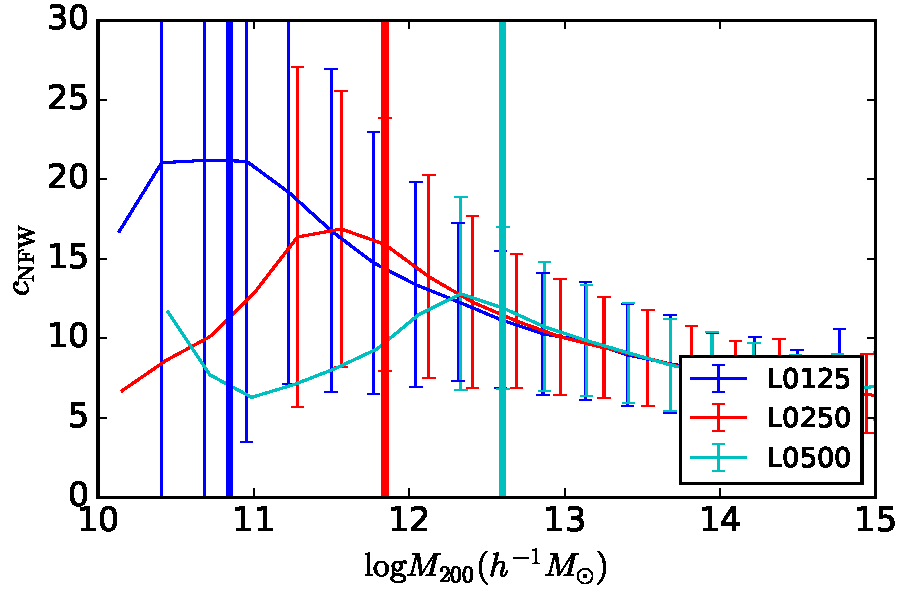
\includegraphics[width=.5\textwidth]{masscut_cNFW_d200.pdf}
\caption{An example of the relationship between the NFW concentration and halo mass for each of our simulations for $\Delta =200$. The chosen lower limit on halo mass for our sample is marked as a blue, red, or cyan line for \simA, \simB, and \simC \ respectively. Note the deviation from a monotonic trend as a result of resolution effects.}
\label{fig:cnfwrelation}
\end{figure}
%--------------------------------------------------------------------------------


%------------------------------------------ Figure for C_V(M)
\begin{figure}
\centering
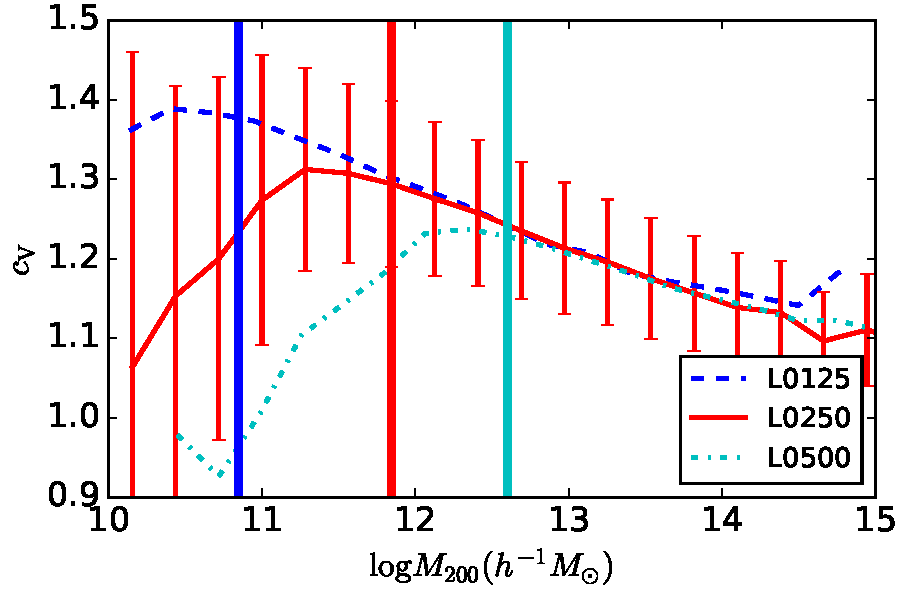
\includegraphics[width=.5\textwidth]{masscut_cV_d200.pdf}
\caption{An example of the relationship between the velocity ratio concentration and halo mass for each of our simulations for $\Delta =200$. The chosen lower limit on halo mass for our sample is marked as a blue, red, or cyan line for \simA, \simB, and \simC \ respectively. Note the deviation from a monotonic trend as a result of resolution effects.}
\label{fig:cvrelation}
\end{figure}
%--------------------------------------------------------------------------------

Figure~\ref{fig:concentrations} shows the relationship between $c_{\mathrm{NFW}}$ and $c_{\mathrm{V}}$ for
quantifying halo concentration on a halo-by-halo basis. Generally the two proxies for concentration are related
to each other in a simple manner with relatively small scatter indicating that these two quantities largely
contain the same information about each halo.

%-------------------------------------------- Figure comparing Cnfw and Cv on a halo-by-halo basis
\begin{figure}
\centering
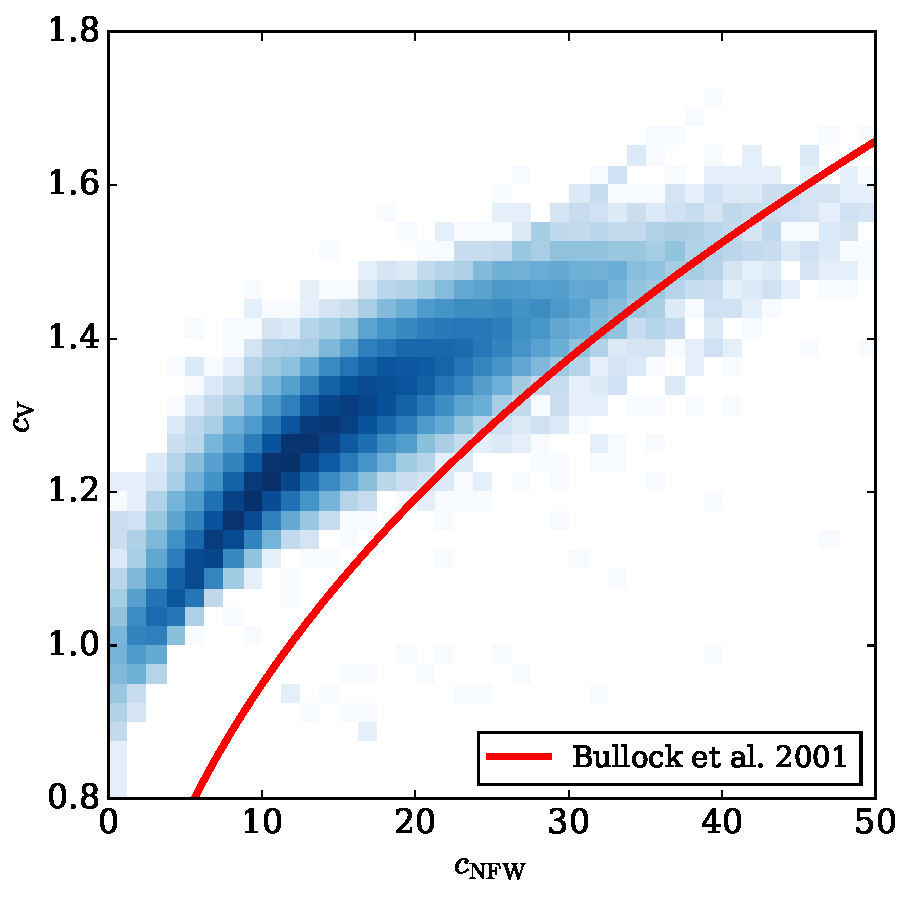
\includegraphics[width=.5\textwidth]{cvvscnfw_relation.pdf}
\caption{
The relationship between the two different marks of concentration, using halos in \simB. The color scale demonstrates the number of halos within a single binning in the concentration space, where redder colors demonstrate where the bulk of halos lie on this relation. 
\arz{This is not sufficiently specific as a caption. For example, you don't say what the color code is or what the color scale is.}
\asv{Hopefully that is sufficient! Unsure how to make a label for the color bar at this time, but looking into remaking this plot. The code may have been on the previous computer, so I'll take a little bit of time to recall how I went through this plot.}
}
\label{fig:concentrations}
\end{figure}
%--------------------------------------------------------------------------------------------------------------------------------

In addition to halo concentrations, we explore halo clustering as a function of a variety of other 
halo properties. We explore halo clustering as a function of halo shape quantified by the ratio of 
the minor and major axes length, 
\beq
s = \frac{c}{a},
\eeq
where $a$ is the major axis length and $c$ is the minor axis length. The mean relations of halo shapes 
as a function of halo mass for $\Delta=200$ is shown in Figure~\ref{fig:srelation} along with the mass 
thresholds selected to ensure that our results are not compromised by resolution.


%------------------------------------------ Figure for s(M)
\begin{figure}
\centering
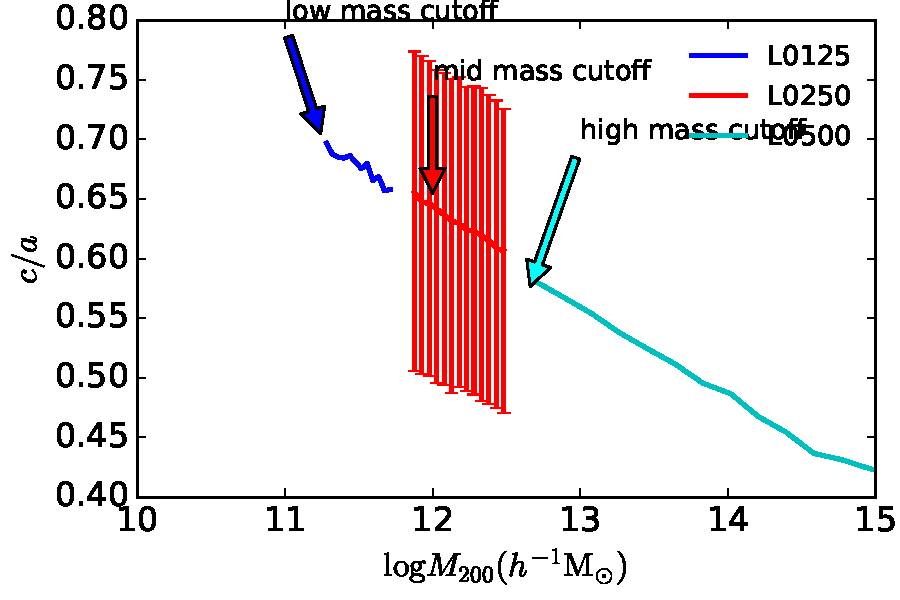
\includegraphics[width=.5\textwidth]{masscut_shape_d200.pdf}
\caption{
An example of the relationship between halo shape and 
halo mass for each of our simulations for $\Delta =200$. The chosen 
lower limit on halo mass for our sample is marked as a blue, red, or 
cyan line for \simA, \simB, and \simC \ respectively. Note the deviation from a monotonic relation as a result of
resolution effects.
}
\label{fig:srelation}
\end{figure}
%--------------------------------------------------------------------------------

We also explore halo clustering as a function of halo spin quantified 
by the spin parameter $\lambda$ as introduced by \citep{peebles69},
\beq
\lambda = \frac{J \sqrt{\lvert E\rvert}}{G M_{\Delta}^{2.5}}
\eeq
where $J$ is the halo angular momentum, $E$ is the total energy of the 
halo, and $M_{\Delta}$ is the mass at the halo radius, $r_{\Delta}$. 
The mean relations of halo spins as a function of halo mas for $\Delta=200$ 
is shown in Figure~\ref{fig:spinrelation} along with the mass thresholds 
selected to ensure that our results are not compromised by resolution.

%------------------------------------------ Figure for lambda(M)
\begin{figure}
\centering
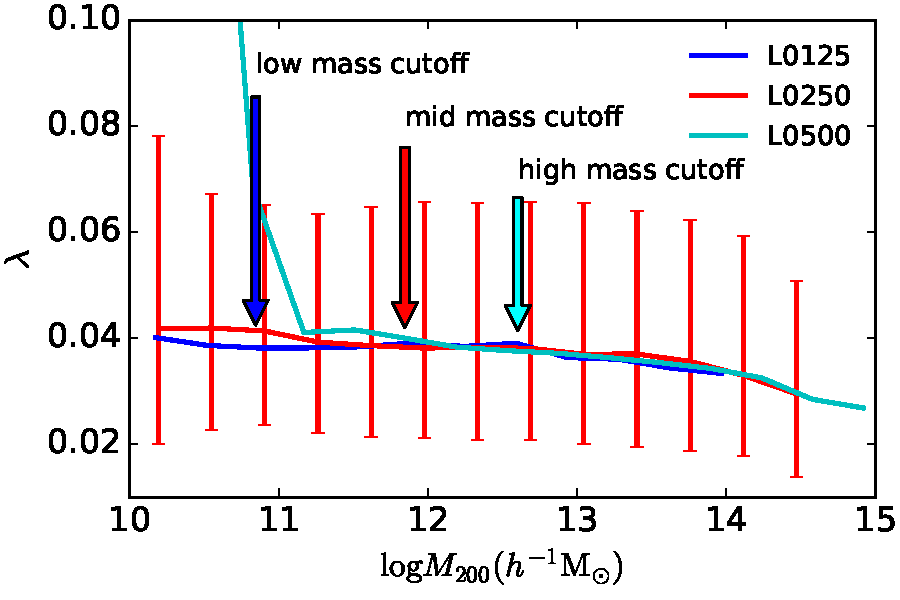
\includegraphics[width=.5\textwidth]{masscut_spin_d200.pdf}
\caption{
An example of the relationship between halo spin $\lambda$ 
and halo mass for each of our simulations for $\Delta =200$. 
The chosen lower limit on halo mass for our sample is marked 
as a blue, red, or cyan line for \simA, \simB, and \simC \ respectively. 
Note the deviation from a monotonic relation as a result of resolution effects.
}
\label{fig:spinrelation}
\end{figure}
%--------------------------------------------------------------------------------

In practice, the mean relations between the various halo properties and the mass thresholds must be determined 
for each combination of simulation, halo property (e.g., $c_{\mathrm{NFW}}$ or $s$), and halo definition (e.g.,
value of $\Delta$). We use thresholds determined by the particular case under consideration so as to ensure that
resolution limitations do not drive any of our primary results. A higher mass threshold means that we do not have
any issues due to halo resolution, but of course, higher mass thresholds reduce statistical power. As an example,
we summarize the mass thresholds we have used for a subset of $\Delta$ values in Table~\ref{table:thresholds}. 
At most values of $\Delta$, the minimum mass thresholds are driven by the requirement that the halo properties do 
not suffer significantly from finite resolution effects; if too many low mass halos are included, the true
relations can be lost in halos which have insufficient numbers of particles for robust statistics on an
individual property.
\arz{Please check the veracity of this last sentence. Some such sentence summarizing the factors that limit our mass cuts should be in the paper.}
\asv{Slightly modifying this statement due to the fact that I think that multiple parameters are brushed up against the lower limits of the mass cuts.}

\arz{In the table, don't ``low mass," ``mid mass," and ``high mass" correspond to the different simulations? For example, low mass corresponds to \simA~and so on? If not, then I don't understand. If so, then you should label each cut by the relevant simulation name as well.}
\asv{We use the various mass cuts across simulations, so I was going for a more general name - e.g. we use high mass on both L0250 and L0500, which allows us to probe if the relation is driven by the simulation size or the actual mass threshold. I can swap out to more specific names though, but I thought that might cause confusion. It seems like we have swapped away from that methodology in the final version, so that might be best.}

%%%%%%%%%%%%%%%%%%%%%%%%%%%%%%%%%%%%%%%%%%%%%%%%%%%%%%%%%%%%%%%%%%%%%%%%%%%%
\begin{table*}
\caption{
Minimum mass thresholds for each of our analyses depending upon the 
value of the overdensity, $\Delta$, used to define the halos. 
In the columns below the values of $\Delta$ we show the minimum 
host halo masses considered in units of $h^{-1}\mathrm{M}_{\odot}$.
}
\vspace*{8pt}
\begin{tabular}{ c c c c c c c }
\hline
\hline
Cutoff Name &  $\Delta=340$ & $\Delta=200$ & $\Delta=100$ & $\Delta=75$ & $\Delta=50$ & $\Delta=10$ \\
\hline
\\{low mass} & {N/A} & $7 \times 10^{10}$ & $8 \times 10^{10}$ & $9 \times 10^{10}$ & $1 \times 10^{11}$ & $2 \times 10^{12}$  \\
{mid mass} & {N/A} & $7 \times 10^{11}$ & $8 \times 10^{11}$ & $9 \times 10^{11}$ & $1.5 \times 10^{12}$ & {N/A} \\
{high mass} & $3 \times 10^{12}$ & $4 \times 10^{12}$ & $5 \times 10^{12}$ & $6 \times 10^{12}$ & $7 \times 10^{12}$ & {N/A} \\
\hline
\hline
\end{tabular}
\label{table:thresholds}
\end{table*}
%%%%%%%%%%%%%%%%%%%%%%%%%%%%%%%%%%%%%%%%%%%%%%%%%%%%%%%%%%%%%%%%%%%%%%

\arz{I would like to see another figure here. I would like to see $M_{200}$ on the x-axis and $M_{\Delta}$ on the y-axis. What should be plotted is the mean $M_{\delta}$ as a function of $M_{200}$ for all halos common to both catalogs. This will be a nice informative plot for the reader and will help the reader to digest the table.}
\asv{Will do using the halo matched catalogs - in progress.}

%-----------------------
\section[]{Halo Clustering as a function of Auxiliary Halo Properties}
\label{section:methodology}
%-----------------------

\arz{I actually don't understand what you are saying in this paragraph. I hope there is nothing special about \simB~? Aren't the mass limits determined as you stated in the previous section for each simulation and for each $\Delta$? If so, why does this all need to be repeated here? Perhaps you can just get rid of this paragraph if you are giving this information in the previous section. That would be my preference for logical flow.}
\asv{Agreed. I think this is probably a repeat at this point. There is nothing special about any given simulation.}

%----------------------------------------------------------
\subsection{Auxiliary Halo Properties}

\arz{I thought that the Duffy et al. paper only looked at concentration? Is this correct? Either way, there is an 
Allgood et al. paper that comprehensively examines this for various halo properties and should be cited here.}
\asv{Found an Allgood paper that is looking at shape, but I'll do a lit search to see if I can't find something else explicit about some of the other parameters}
Another well known effect is the scaling of our properties as a function of halo mass, as well demonstrated
within the literature \citep{allgood06, duffy08, despali16}. We are interested in studying the clustering behavior of halos
as a function of properties other than mass. As mass is the dominant halo property correlated with halo
clustering strength and environment, we refer to the additional properties that we study as 
``auxiliary halo properties" (those properties other than mass, such as concentration $c_{\rm NFW}$ or shape
$s$). 

Most contemporary cosmological $N$-body simulations, including the set that we study here, 
do not have a sufficiently large number of halos to make isolating halos of fixed mass, and then further 
splitting these halos by an auxiliary property, a powerful method with which to study the dependence of 
clustering on auxiliary properties. Consequently, we study this phenomenon using halo samples 
selected according to minimum mass thresholds. To do so, we remove the mass dependence of 
the auxiliary properties as follows. 

We take all host halos of interest and sort them by their halo mass, $M_{\Delta}$. 
Ten equally spaced bins of log mass are generated to sort these halos into, ensuring that no bin has one or zero
halos. The mean value of each halo property is calculated within each bin, and subtracted from the recorded value
for each halo in the bin. This removes the strong mass trend in each of these properties, allowing us to avoid a
need to just look at halos at some fixed mass. We use these mass-dependence removed concentrations, shapes, and
spins in all calculations throughout the paper.
\asv{More detail is given. I'm not necessarily comfortable with the current ten bin situation and could conceivably switch back to equally populated bins, which allows for more total bins with halos to look at, but unevenly spaced in log mass.}
\arz{First, you need some equations here. It is unclear to the reader what the word ``normalize" means in this context. YOU MUST provide enough information so that someone with access to these simulations could reproduce your calculations. Also, you don't give important details. How many are in the ``equal populations" for example. You may also want to add an additional paragraph speculating briefly on other ways to remove the gross mass dependence. You must also say explicitly that we use the mass-dependence-removed concentrations, shapes, and spins in all following calculations. This might not be the exact wording you want to use, but you can decide what you want to call these things.}

\arz{Flesh this out a bit. See the discussion in Wechsler et al. 06 as a model. The specific values of the thresholds need to be given} 
\asv{Slight change - following Wechsler et al 06 does not ever put a specific limit on subhalo velocity and instead places a limit on the ratio between the subhalo velocity and the host velocity as the prime limit. Just making sure that lines up well.}

To mitigate the correlation between halo mass and satellite number, 
we follow the prescription of \citet{wechsler06}. We select only host halos 
with $v_{\mathrm{max,host}} \ge 240 \ \mathrm{km \ s}^{-1}$ in addition to the previous mass cuts. 
This ensures that the satellite counts will be minimally affected by finite resolution. We then select subhalos
from the sample based on the criteria that the ratio $v_{\mathrm{max,sub}} / v_{\mathrm{max,host}} \ge 0.3$. The
subhalo velocity function is a very nearly self-similar function \citep{zentner05} \arz{Cite Zentner, Berlind et
al. 2005 and references therein on this point.}, so that scaling subhalo $v_{\mathrm{max,sub}}$ by host
$v_{\mathrm{max,host}}$ in this way eliminates the gross mass dependence of satellite number. The value chosen
for this ratio has been adopted such that all host halos that make the above cut contain, on average, one
selected satellite halo. As a final selection cut, for each host halo, only the number of subhalos within the
radius $R_{\Delta}$ of the host are counted. 

\arz{In the earlier draft, the preceding paragraph had a logical flow that made it 
very difficult to follow the steps in the calculation. If you think about it for a minute, the 
important pieces are: (1) we quantify subhalo size with $v_{\mathrm{max,sub}}$ because 
it is more robustly measured than subhalo mass; (2) there is a minimum $v_{\mathrm{max,sub}}$ 
that we can aspire to reach because of resolution; (3) we quantify subhalo number by scaling 
subhalo size relative to host size, $v_{\mathrm{max,sub}}/v_{\mathrm{max,host}}$, because this 
scales out the gross dependence of subhalo number count on host halo size; (4) we must choose 
host halos that are sufficiently large that the contain, on average, a few subhalos above our 
minimum subhalo $v_{\mathrm{max,sub}}$. These considerations completely specify the 
cuts on $v_{\mathrm{max,sub}}$ and $v_{\mathrm{max,host}}$. Please make sure these 
elements of the logic are clear to the reader.}
\asv{I think the steps should be clear at this point? Let me know if not.}

%---------------------------------------------------------------
\subsection{Clustering Statistics}

We assess the influence of assembly bias on two-point statistics of host halos. In order to do so, we 
study both the standard two-point correlation functions of halos selected by properties other than mass 
(e.g., the auxiliary properties concentration, shape, and spin) as well as halo mark correlation functions
(MCFs). MCFs quantify the manner in which a halo property (the ``mark") correlates among halo pairs as a function
of the distance between the pairs. Absent halo assembly bias, halo marks are uncorrelated among pairs. 
MCFs have been used in several previous papers to quantify environmental dependence of halo 
properties other than mass \citep{sheth04, harker06, wechsler06, mao15} \arz{I think there are also a couple of 
Sheth papers that should be cited here, maybe more}. 
For a specific halo property, or mark $m$, we use the MCF normalization of \citet{wechsler06}, namely 
\beq
\mathcal{M}_m(r) \equiv ( \langle m_1 m_2 \rangle_p (r) - \langle m \rangle^2 / \mathcal{V}(m),
\eeq
where $m_{\mathrm{i}}$ is the value of the mark for halo $\mathrm{i}$, $\langle m \rangle$ is the mean of the
mark, and $\mathcal{V}(m)$ the variance of the mark. The notation is intended to indicate that the average is
taken over all pairs of halos separated by a distance $r$. In the absence of any correlation between a halo
property and the halo having a neighbor a distance $r$ away, $\mathcal{M}_m(r) = 0$. Deviations of the MCF from
zero indicate such correlations exist and the size of the $\mathcal{M}_m(r)$ gives the excess of the mark among
pairs compared to the one-point mean of the mark $\langle m\rangle$ in units of the one-point variance.


It is necessary to assess statistical fluctuations in the statistics that we measure in these simulations in
order to determine the significance of the signals. For two-point correlation functions, we determine the
covariance of the measurement through jackknife resampling of the eight octants of the simulation cube. We assess
the statistical significance of the MCFs by randomly re-assigning each of our marks to the halos in the sample. 
We then compute the MCF of these randomized marks. As the mark re-assignment is random, 
the MCF computed on these re-assigned marks {\em cannot} exhibit any 
environment dependence other than that induced by statistical fluctuations. 
We perform this reassignment 400 times and approximate a $2\sigma$ error region by 
the span of the MCF between our 10$^\mathrm{th}$ lowest and 10$^\mathrm{th}$ highest (that is the
390$^\mathrm{th}$ if the MCFs were sorted in ascending order) values of the MCF. In the event that there are no
environmental correlations with halo auxiliary properties, the MCFs measured in the simulations would fall within
this error band $95\%$ of the time. 


\arz{The sentences immediately below this comment can be removed. Also, not a wise idea to 
lock yourself into 20\% in the text. There is absolutely nothing special about 20\%. In fact, it 
would be interesting to see if things change as this percentile changes, perhaps try 50\% and 
10\%. We should at least know what those figures look like before proceeding to publication, 
so you should make them even though we likely won't include them in the main text of 
the paper. It could be very informative and will almost certainly be useful when giving talks.}
\asv{Removed - the new framework with halo tools makes it easier to test any cut that we want in short order as well.}



%----------------------------
\section[]{Results}
\label{section:results}
%----------------------------

\arz{We don't need to reiterate all of this stuff about the mass cuts. Just make sure the discussion in the simulations section is complete and then we can move forward. Again, I suggest changing the names of your cuts. It would be great if they can signify something either about the ACTUAL MASS involved in the cut or the simulation or possibly BOTH! Perhaps you can say the ``L0125" cut and so on? 
If you get everything specified in the simulation section, then this paragraph is completely unnecessary.}
\asv{Removed - still debating how to name these cuts.}
\arz{It seems to me that we DO include \simC~!! Even if we don't we should. Let's treat each simulation as simply sampling a different range of halo masses. That is the most useful way to proceed.}
\asv{Also removed - this was leftover from the old plots, before L0500 was included in all the plots.}

%-----------------------------------------------
\subsection{Correlation Functions}
\label{sub:cfresults}

\arz{Fix up and fill in numbers as needed, but follow this general format.}
We begin by studying the correlation functions of halos in our mass threshold samples, sub-selected by auxiliary
properties. Figure~\ref{fig:cc_cfcompare} exhibits the difference between the clustering strength of halos in the
$20^{\mathrm{th}}$ percentile highest concentrations and the halos with the halos that have the
$20^{\mathrm{th}}$ percentile lowest concentrations as a function of the overdensity parameter $\Delta$, used to
define the halos. First, it is clear that clustering strength generally depends upon the auxiliary properties of
halos at all halo mass thresholds. Second, it is clear that the strength and sign of assembly bias is 
strongly mass dependent, a result that agrees with the significant previous literature on halo assembly bias
\citep{wechsler02, gao05, zentner07, wechsler06, harker06, croton07, dalal08, mao15, sunayama16}\arz{Cite all the usual 
papers here, Gao, Wechsler, Harker, Zentner07, Dalal07, probably several more.}\asv{I think that is most of the
usual suspects, but I'll do a double check for more important ones!} At relatively low mass (the L0125 panel, 
$M_{200} > 7 \times 10^{10} \hMsun$), high-concentration halos are considerably more strongly concentrated 
than low-concentration halos using the more 
conventional $\Delta = 200$ definition for halos. At somewhat higher halo masses (the L0250 panel, $M_{200} > 7
\times 10^{11} \hMsun$), this difference is markedly reduced. Finally, for the highest mass halos that we have
the capability of studying (the L0500 panel, $M_{200} > 4 \times 10^{12} \hMsun$), the effect is of opposite
sign; low-concentration halos are more strongly correlated than high-concentration halos.

\asv{Added a little bit of language to your version to include the new results for the new results.}
\arz{The language in this paragraph is way too loose and not sufficiently clear or professional. What does it mean to be a ``reasonable" mass range, for example? I'll attemp to clean it up. Try to follow this model in your writing. Compare my version:}
Focus first on the middle panel of Fig.~\ref{fig:cc_cfcompare}. In this panel, corresponding to the 
\simB~mass threshold, the difference in large-scale clustering between high- and low-concentration halos 
is dramatically reduced for a halo definition with $\Delta=75$. Further decreasing $\Delta$ leads to
concentration-dependent clustering of opposite sign. Comparing the differing clustering 
strengths across the three panels of Fig.~\ref{fig:cc_cfcompare}, it is clear that this is not a universal
conclusion. For low-mass halos, very low values of $\Delta$ (and correspondingly large definitions of halo radii,
as $R_{\Delta} \propto \Delta^{-1/3}$) are necessary in order to mitigate the concentration dependence of halo
clustering; while dramatically reduced for a halo definition with $\Delta \approx 10$, there is a potential
danger of systematic effects related to halo finding algorithms at such an extreme value. Conversely, for higher
mass halos (the L0500 panel), values of $\Delta \approx 200$ yield little concentration-dependent clustering. In
this case, decreasing $\Delta$ (increasing $R_{\Delta}$) results in significantly {\em increased} concentration
dependent halo clustering. The reasons for these changes is of interest and we return to interpreting these
results below.

Notice that in all panels of Fig.~\ref{fig:cc_cfcompare}, the effect of concentration-dependent clustering is
scale-dependent. Moreover, the effect is scale-dependent for all values of $\Delta$. In these cases, simply
defining halos with a different value of $\Delta$ does not suffice to eliminate concentration-dependent
clustering on all scales. In this discussion and throughout, we focus primarily on the large scale clustering,
which we take to mean clustering on scales significantly larger than the radii, $R_{\Delta}$ of the halos in our
samples.

\arz{Given how the correlation functions look, shouldn't we include results for $\Delta<50$, for the L0125 results? The effect is continuous so it looks like it would be removed with a smaller value of $\Delta$, say $\Delta \approx 20$. I think you have run this already, so no reason to leave it out. I say this is a must for moving forward with publication.} 
\asv{Definitely in the works for L0125! Just finishing up some runs in order to sort things out.}

\arz{On another note, did you ever compute these things for finer spacing of $\Delta$? For example, it looks like $\Delta \approx 70$ is going to work better than $\Delta=75$. It's OK if you haven't, but let me know! I thought we had discussed this. } 
\asv{We have some finer spacing to investigate from previous runs.}

\arz{For the high-mass, L0500, cut, did you try any $\Delta>200$, maybe $\Delta=210$ or so? This is not really necessary, I'm just curious how this looks.} 
\asv{We also have finished a $\Delta = 340$ run of this to examine as necessary.}


\begin{figure}
	\centering
	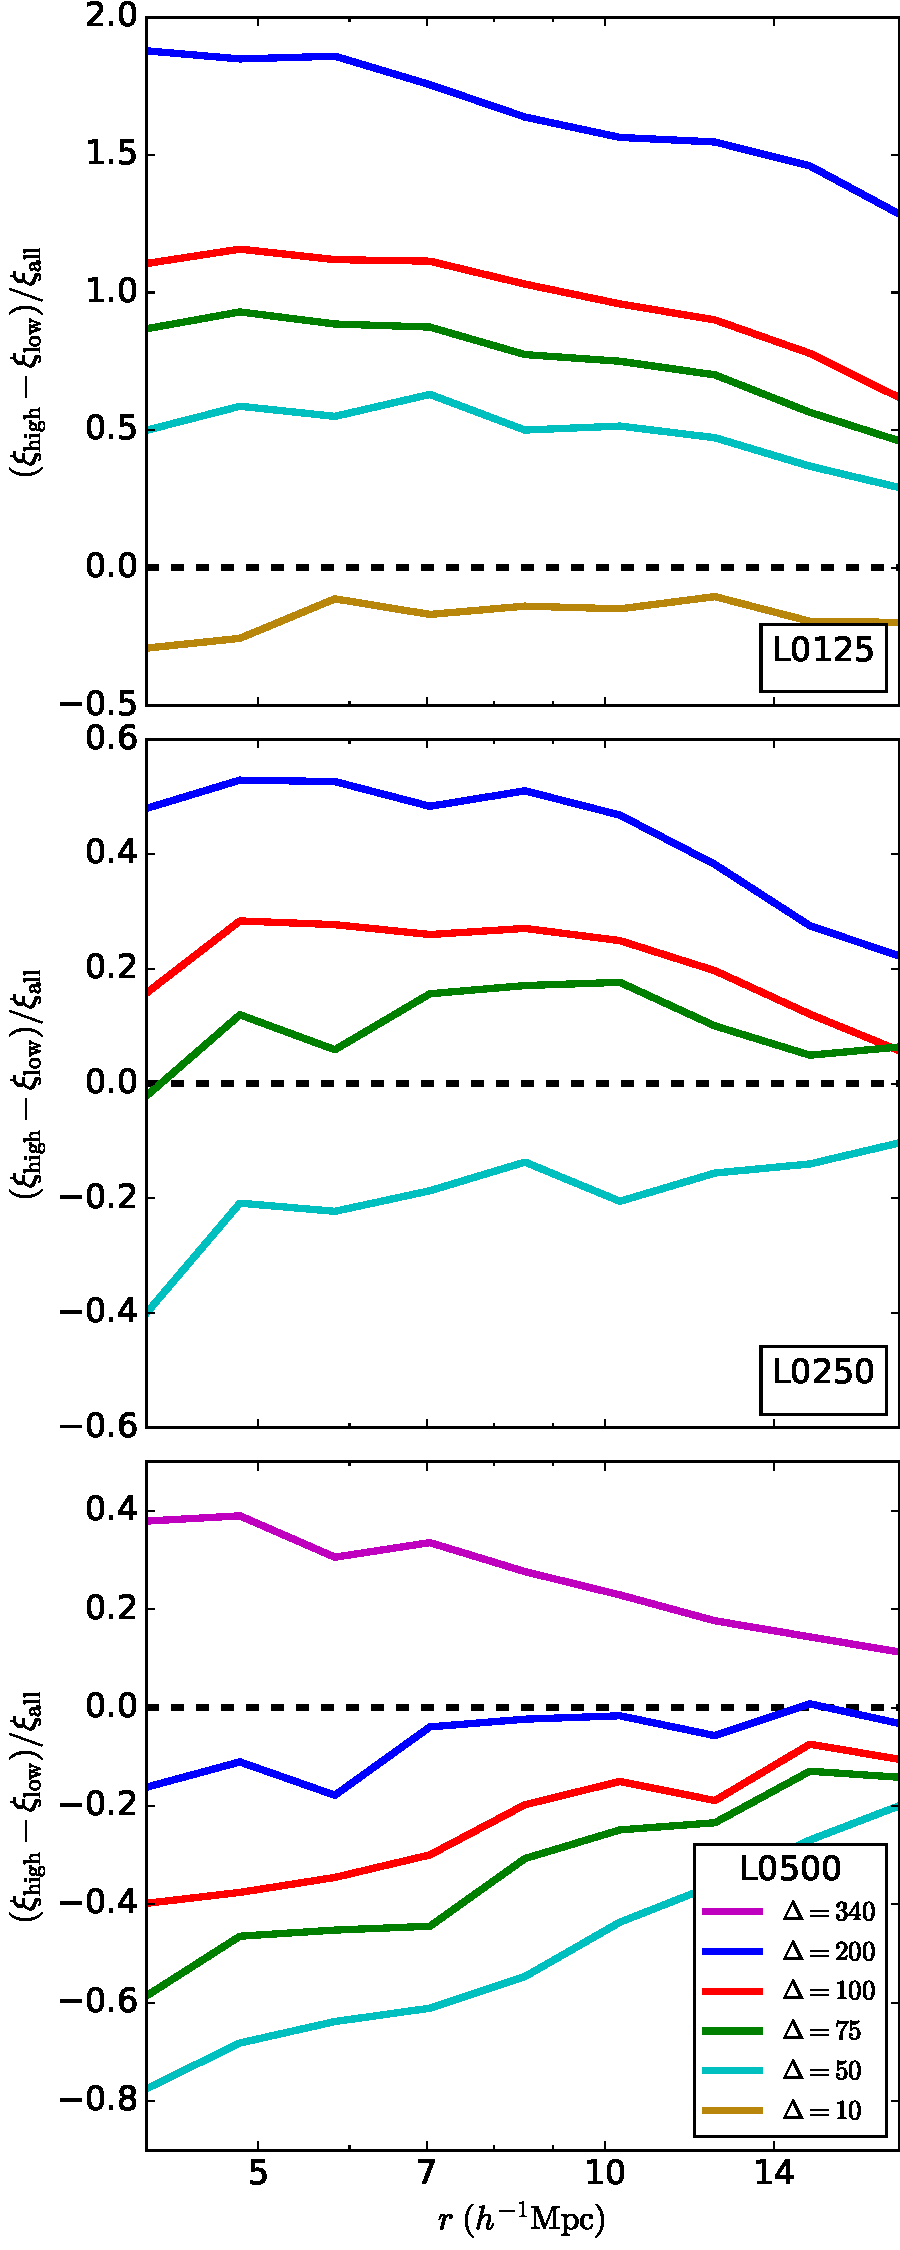
\includegraphics[width=.4\textwidth]{all_cfcompare_cnfw.pdf}
	\caption{
The difference of the correlation function for only the top 20\% most concentrated halos and the bottom 20\% in concentration, normalized by the overall correlation function of the entire sample. From top to bottom we show the results for the `low mass', `mid mass', and `high mass' cutoffs. \asv{May still need error bars, depending on how clean we want the overall image, but should be quick enough to whip together.}
}
	\label{fig:cc_cfcompare}
\end{figure}

\arz{I assume that if you made the same plot for $c_V$ we would reach the same basic conclusions as for $c_{NFW}$? If this is so, then you need to add a specific statement in this regard to the end of the discussion above. In this case, no new figure would be needed. If not, then you need to show the figure.}
\arz{In this subsection, I advocate at least one and perhaps two new figures. First, can you make an analogous plot to Fig.~\ref{fig:cc_cfcompare} that shows some other property, such as shape or spin? This would be a nice addition for completeness. Second, what would happen if you used 50\% or 10\% cuts on concentration? Would we reach nearly the same conclusions? If so, then you do not need to show the plots explicitly. However, in this case, you DO need to state explicitly that this is the case. In other words, you need to state the the broad conclusions we reach are roughly independent of the specific percentiles that we use to select halos so that showing results for a variety of different percentiles doesn't add very much to the discussion. It is also possible that selecting on a different percentile yields an entirely different conclusion. I don't suspect that this will be the case, but it is possible. If that happens, then you need to show an example of such a figure for, say, concentration.}
\asv{These have all been tested at this point. They do not offer any unique conclusions, so I am uncertain if they want to be included beyond the concentration one, which shows the equivalence of the two methods.}

%-----------------------------------------------------------------
\subsection{Mark Correlation Functions}

\begin{figure}
	\centering
	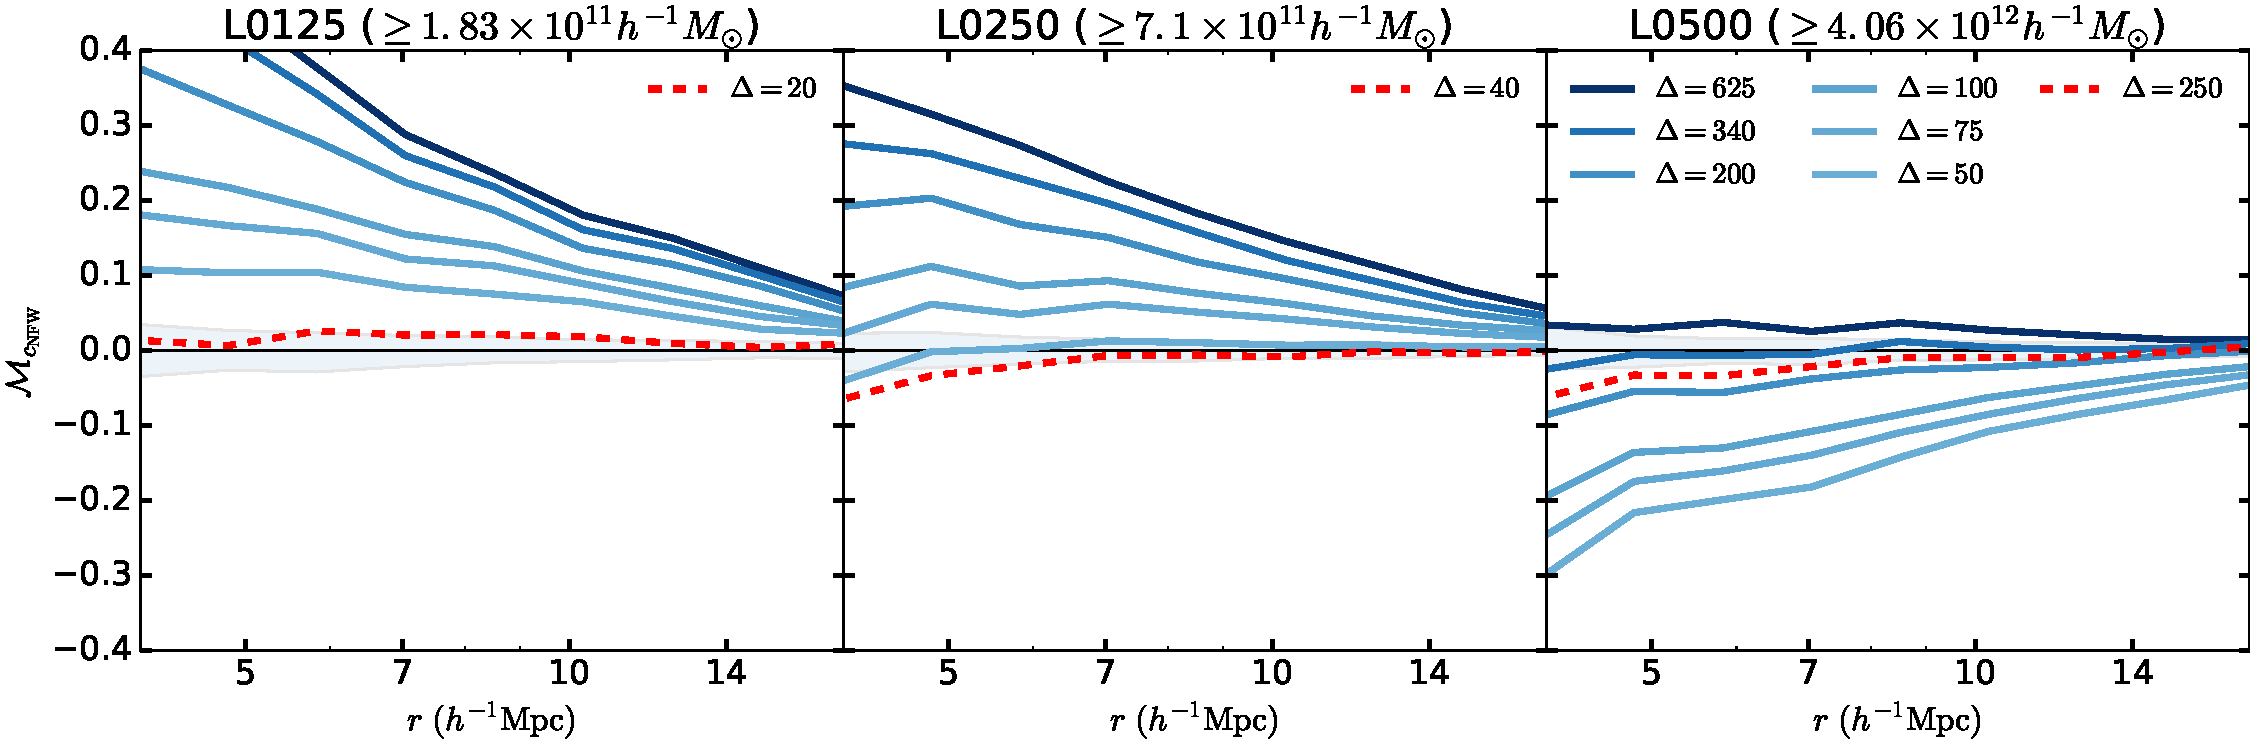
\includegraphics[width=.4\textwidth]{all_mcf_cNFW.pdf}
	\caption{
The marked correlation function for the concentration defined according to the NFW profile. From top to bottom we show the `low mass', `mid mass', and `high mass' cutoffs. The shaded bands represent 2-sigma confidence regions generated by randomization of the marks.
}
	\label{fig:cc_mcf_cnfw}
\end{figure}


We now move toward a discussion of halo assembly bias as diagnosed by MCFs. 
MCFs have the advantage that it is not necessary 
to specify particular auxiliary property subsamples, such as the percentiles above, 
in order to assess assembly bias.\footnote{Of course, this comes at the cost of averaging 
over all values of the auxiliary properties. Using MCFs it is not evident if the assembly bias effect is a smooth
function of the auxiliary properties, dominated by the tails of the auxiliary property, or has some more complex
dependence upon the auxiliary property. Our results in \S~\ref{sub:cfresults} suggest that assembly bias is a
fairly smooth function of the auxiliary properties.} 
The NFW concentration, $c_{\mathrm{NFW}}$, MCF is shown in Figure~\ref{fig:cc_mcf_cnfw}. 
The shaded bands in the figure delineate the statistical fluctuations in MCFs induced by 
finite sampling as discussed in the previous section. Qualitatively, 
Fig.~\ref{fig:cc_mcf_cnfw} exhibits the same features that are evident in 
Fig.~\ref{fig:cc_cfcompare}: more concentrated halos are significantly more clustered in 
the low-mass L0125 halo sample; concentration-dependent halo clustering weakens and 
reverses sense as halo mass increases, consistent with work on assembly bias by \citet{sunayama16}; for the 
L0250 sample with $\Delta=70$, the large-scale concentration dependence of halo clustering has been reduced so as to 
be consistent with zero within the statistical limitations of the simulation. \arz{Again, it seems like we need a 
$\Delta <50$ line for L0125. If possible, it would be great if we could put a $\Delta>200$ line 
on this plot for the L0500 simulation.}


Figure~\ref{fig:cc_mcf_cV} is a similar plot for the velocity-defined concentration, $c_{\mathrm{V}}$ MCF. 
This figure exhibits qualitatively and quantitatively similar features to Fig.~\ref{fig:cc_mcf_cnfw}, a 
fact that is not surprising given that we already know that $c_{\mathrm{NFW}}$ and $c_{\mathrm{V}}$ 
quantify largely redundant information about their halos.

%---------------------------------------------------
\begin{figure}
	\centering
	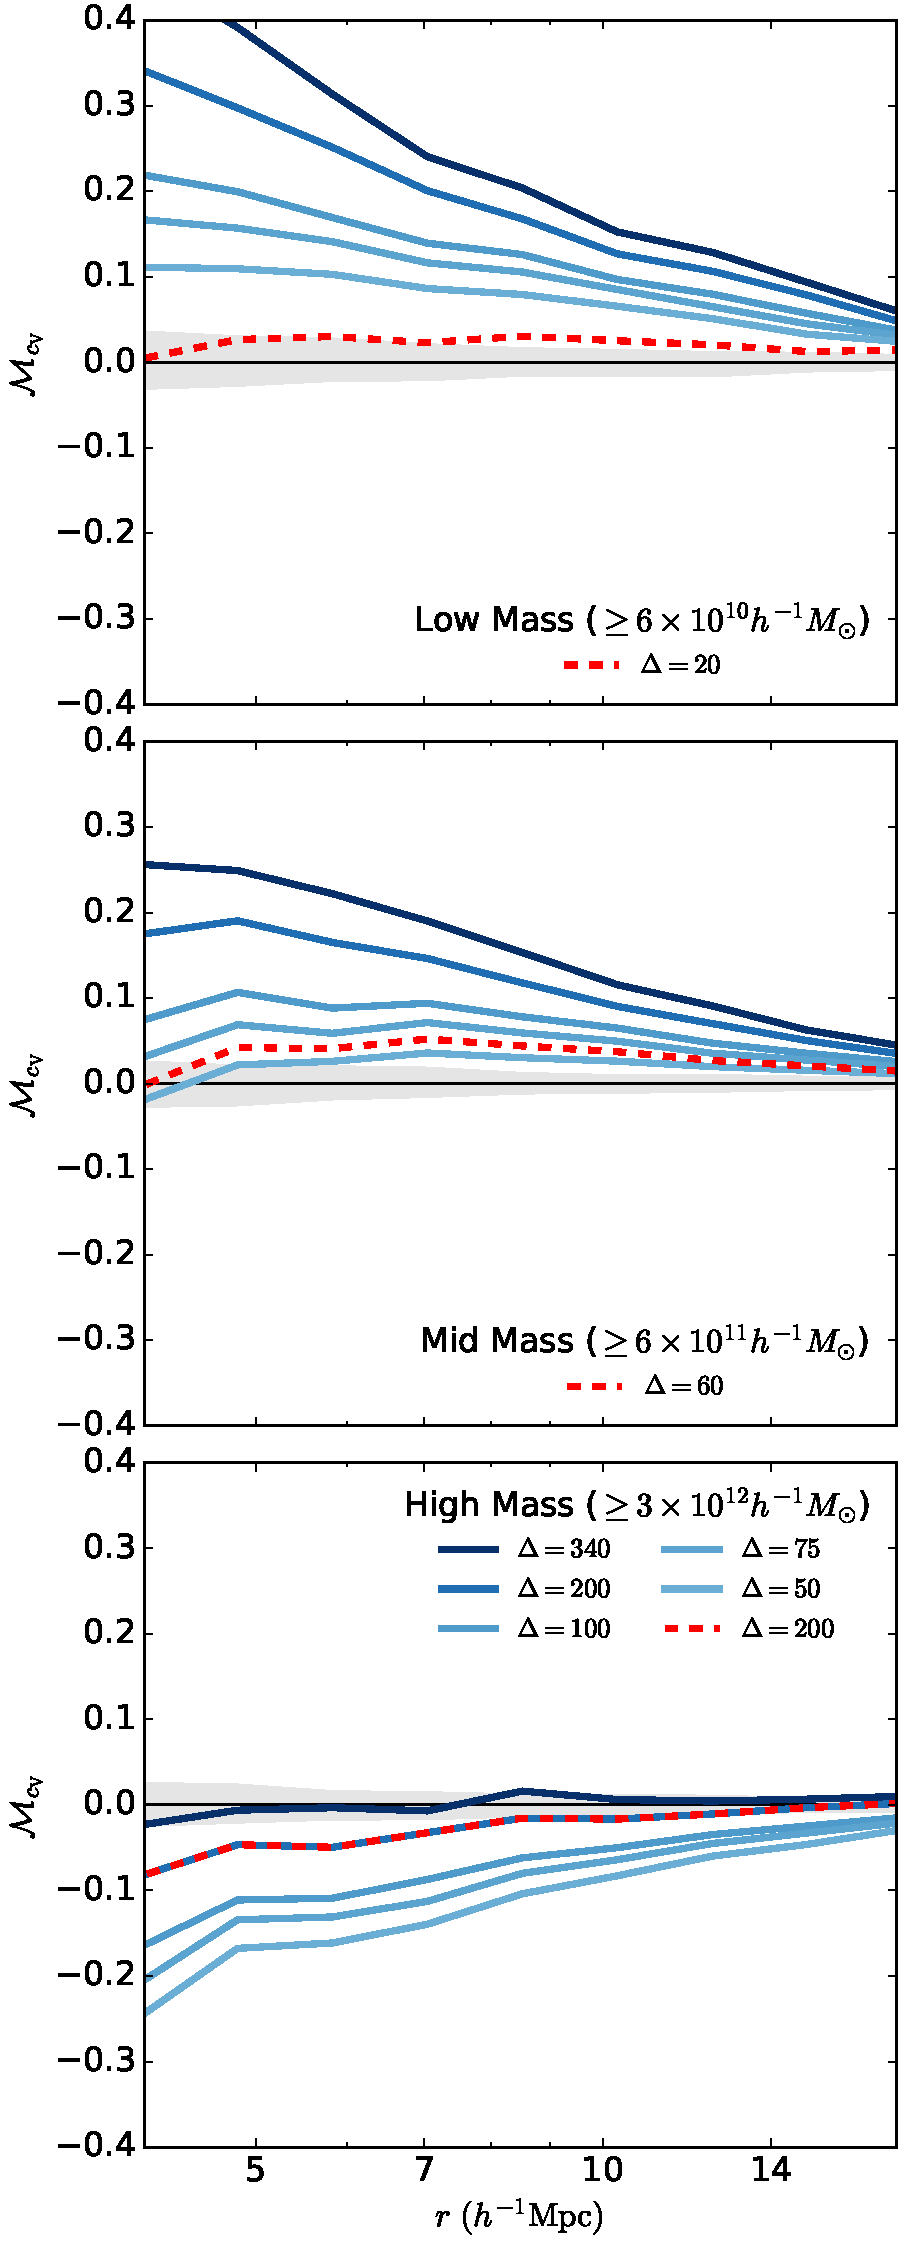
\includegraphics[width=.4\textwidth]{all_mcf_cV.pdf}
	\caption{The marked correlation function for the concentration defined according to the velocity ratio. From top to bottom we show the `low mass', `mid mass', and `high mass' cutoffs. The shaded bands represent 2-sigma confidence regions generated by randomization of the marks.
}
	\label{fig:cc_mcf_cV}
\end{figure}
%---------------------------------------------------

Moving on from concentrations, Figure~\ref{fig:cc_mcf_s} illustrates MCFs in which the mark is the shape
parameter, $s$, of the halo. The environmental dependence of shape parameter is distinct from that of
concentration in a number of ways. Notice that at all masses and at all halo definitions, less spherical halos
(halos with smaller $s$) are more strongly clustered. Furthermore, decreasing $\Delta$ (increasing halo radius)
only serves to increase this environmental dependence in all cases. This is indicative of halo shapes being
driven by structure on scales larger than halo radii, in particular $R_{200}$, and is not entirely surprising
given our significant amount of knowledge of the filamentary nature of large-scale structure. \arz{If possible, a
line here with $\Delta \gg 200$. Seems like it could be instructive, let me know if this is going to take a long
time or be very onerous.}\asv{Added and continues the trend in the direction as expected. Note reversal in
monotonic relationship for lowest mass objects though. Looking over the cuts, this may imply that the mass cuts
are not aggressive enough for the shape mark, though. Vega et al 2016 paper suggests this is the case.}


The spin MCFs are shown in Figure~\ref{fig:cc_mcf_spin}. Qualitatively, spin-dependent halo clustering is 
quite similar to shape-dependent halo clustering. Halos of high-spin cluster more strongly than halos of 
low-spin. \arz{Search the literature, particularly Brandon Allgood's papers and Andreas Faltenbacher whose 
names come to mind, for spin-dependent assembly bias. I'm trying to figure out if yours is the first paper 
to point this out.}\asv{Need to track down all the specific citations, but after changing our normalization
method, it seems to match up better with existing texts.} Likewise, increasing halo radii by decreasing $\Delta$
in halo definitions only drives spin-dependent halo clustering to be stronger.

%---------------------------------------------------
\begin{figure}
	\centering
	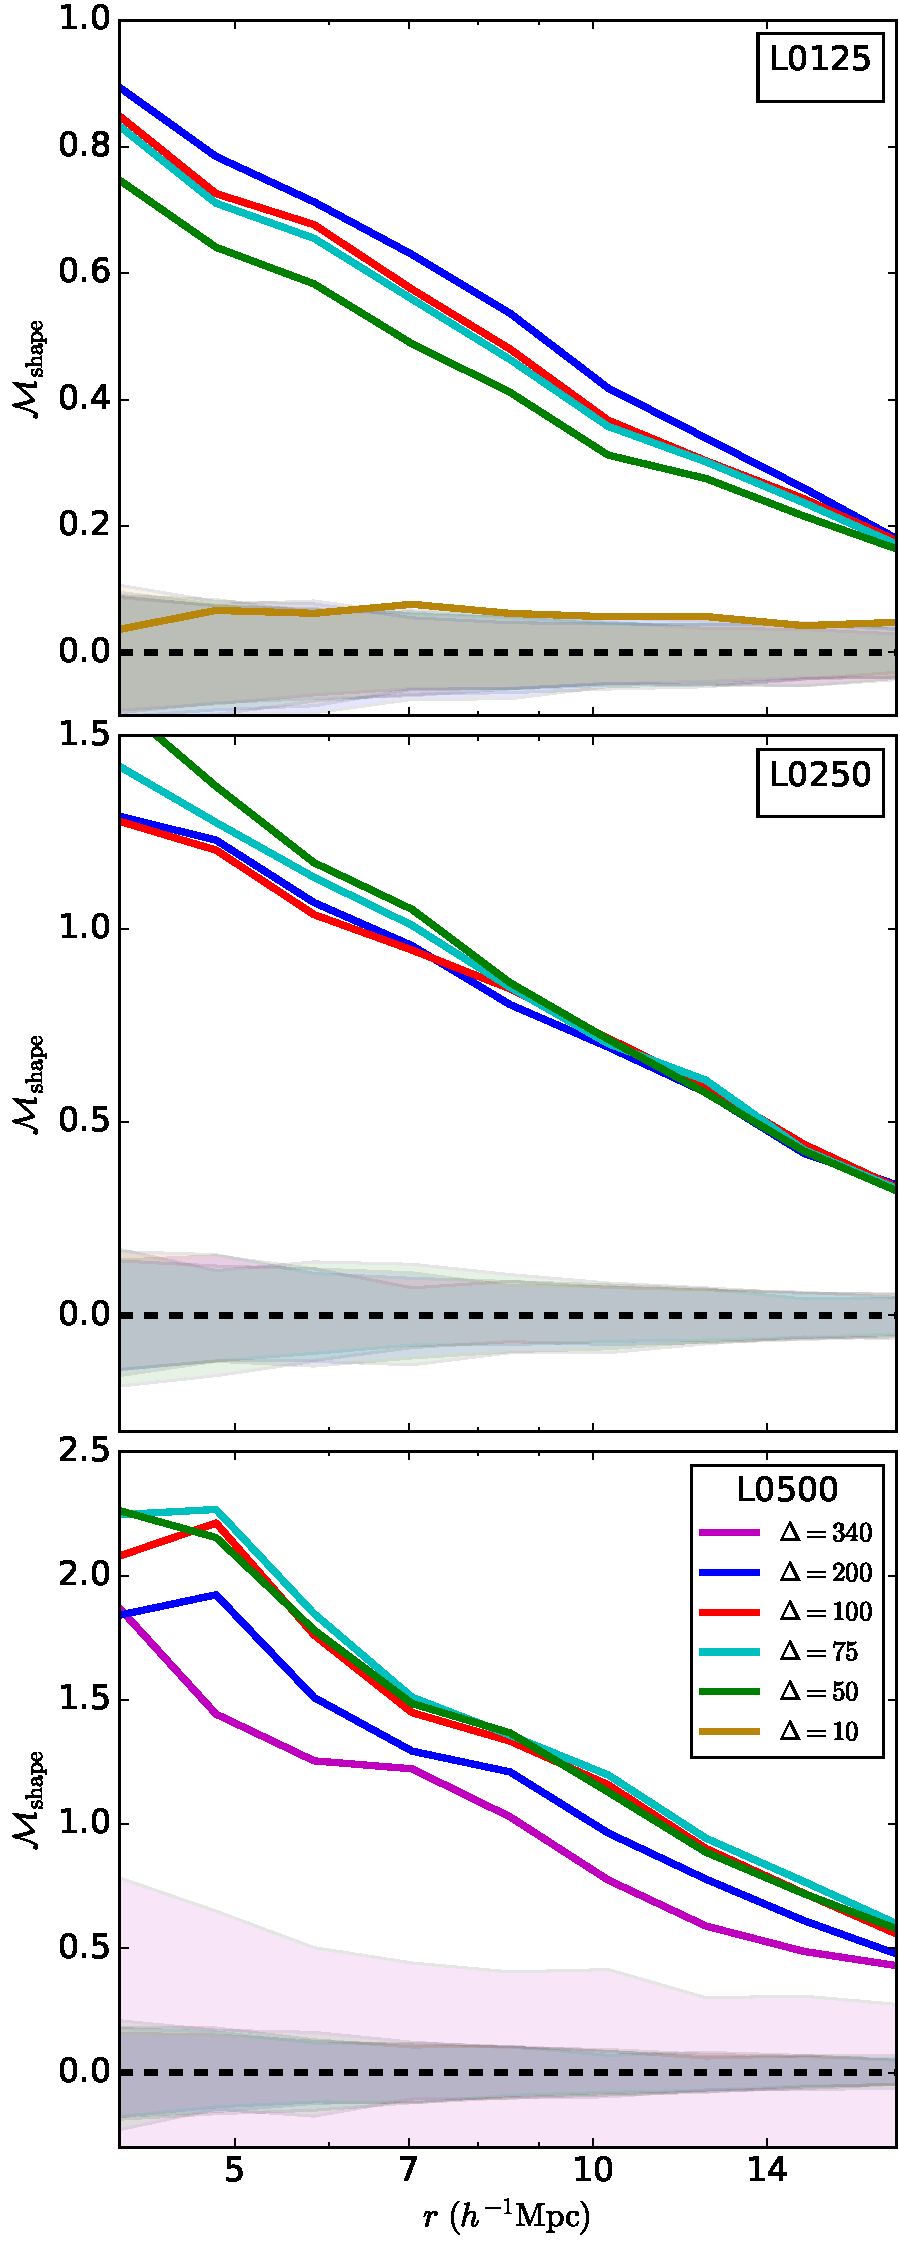
\includegraphics[width=.4\textwidth]{all_mcf_shape.pdf}
	\caption{
	The marked correlation function for the shape of the halo. From top to bottom we show the `low mass', `mid mass', and `high mass' cutoffs. The shaded bands represent 2-sigma confidence regions generated by randomization of the marks. \asv{it is possible that this is driven by insufficiently aggressive resolution cuts. This may drive us to do separate mass cuts for each mark - vexing, but should be feasible in the new framework.}
}
	\label{fig:cc_mcf_s}
\end{figure}
%--------------------------------------------


%---------------- spin MCF
\begin{figure}
	\centering
	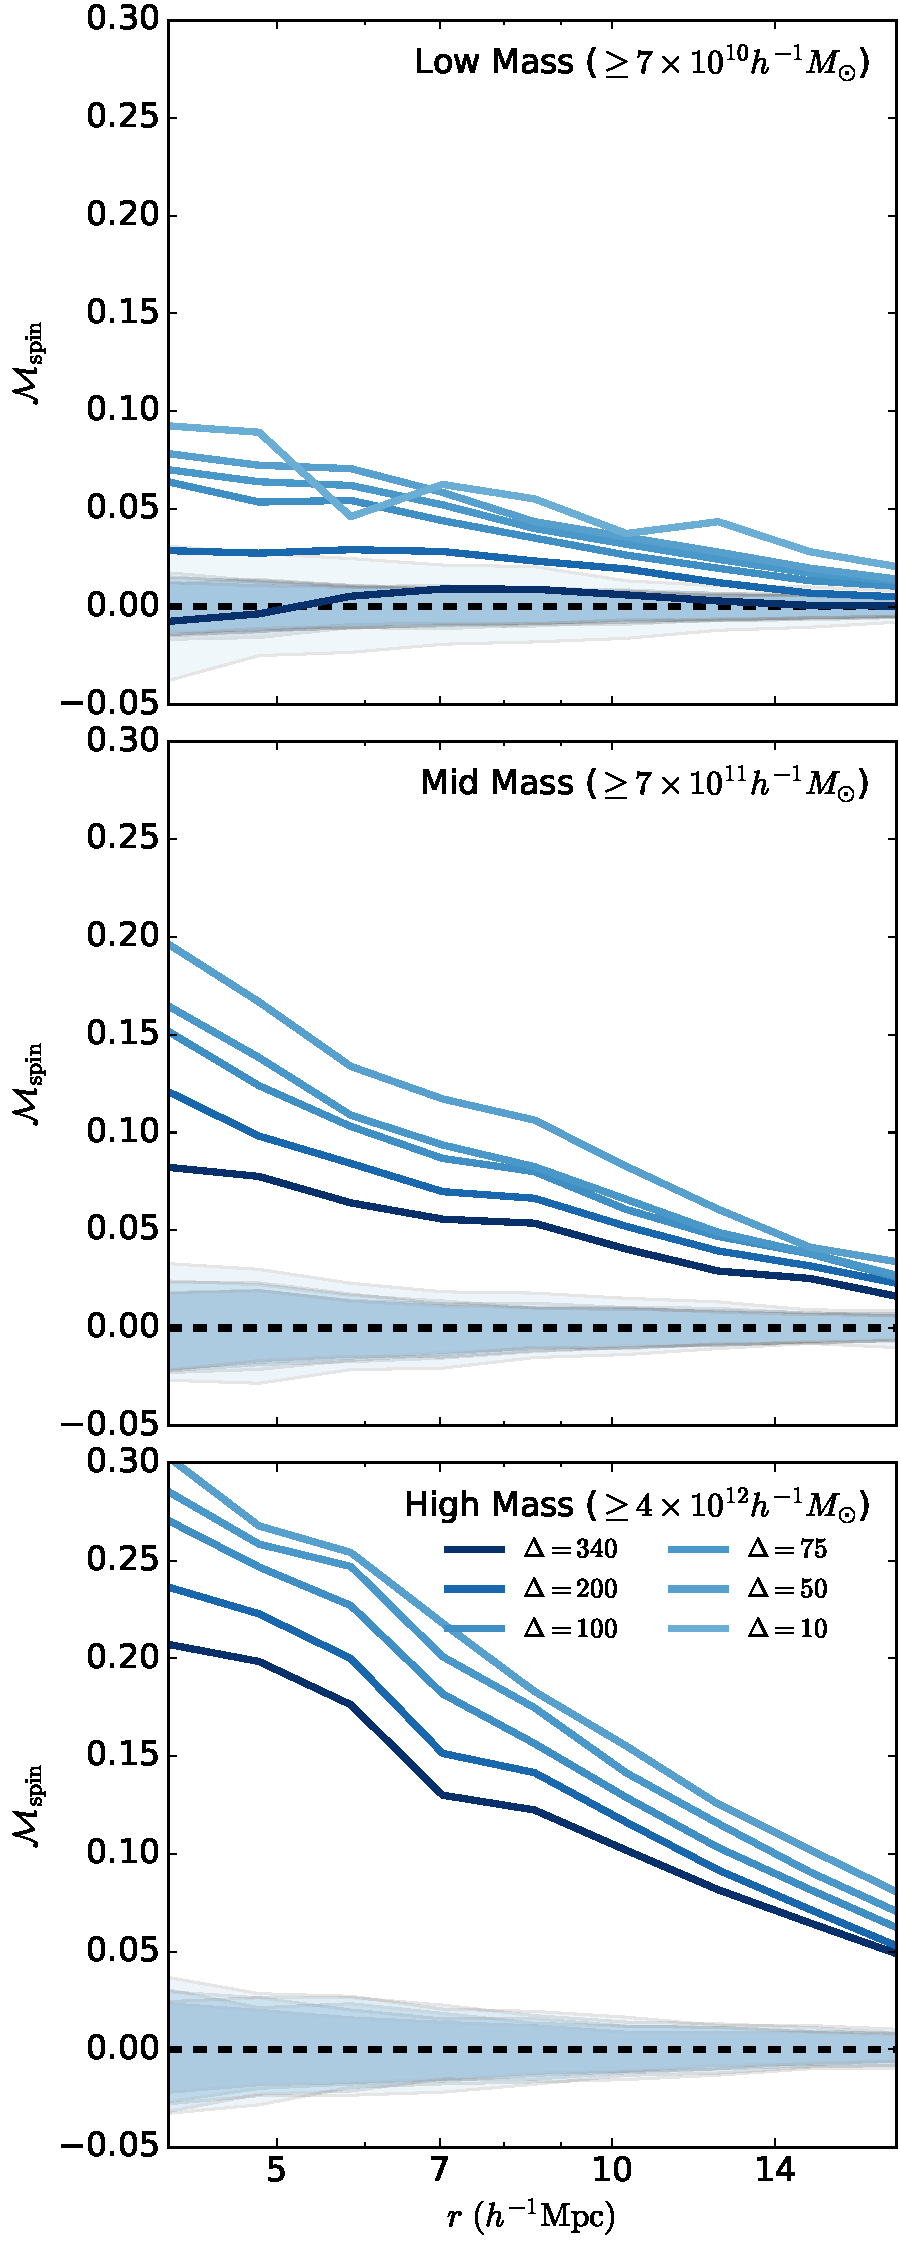
\includegraphics[width=.4\textwidth]{all_mcf_spin.pdf}
	\caption{The marked correlation function for the spin parameter of the halo. From top to bottom we show the `low mass', `mid mass', and `high mass' cutoffs. The shaded bands represent 2-sigma confidence regions generated by randomization of the marks.
	}
	\label{fig:cc_mcf_spin}
\end{figure}
%-------------------------------


%----------------- satellite number MCF
\begin{figure}
	\centering
	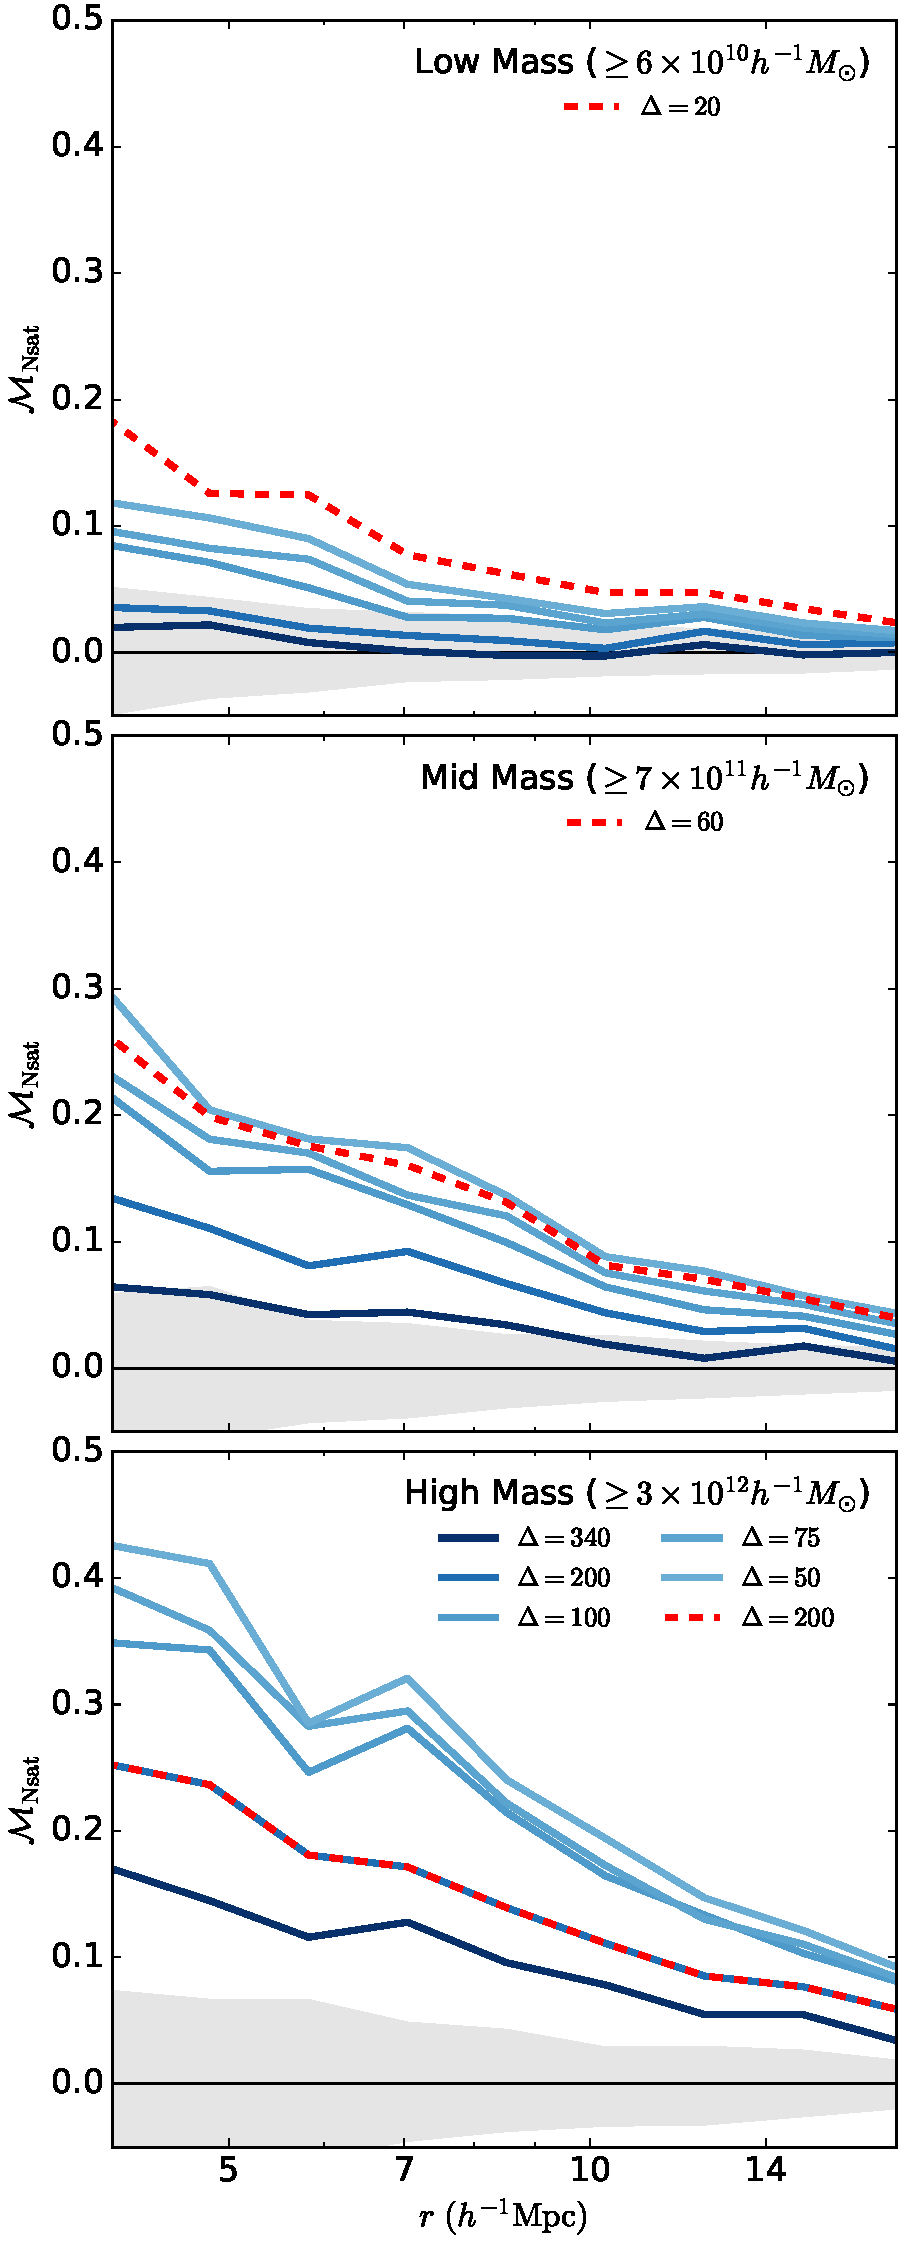
\includegraphics[width=.4\textwidth]{all_mcf_nsat.pdf}
	\caption{The marked correlation function for the number of satellites for a host halo. From top to bottom we show the `low mass', `mid mass', and `high mass' cutoffs. The shaded bands represent 2-sigma confidence regions generated by randomization of the marks.	}
	\label{fig:cc_mcf_nsat}
\end{figure}
%-------------------------------------------------------------------------------------------


The clustering of halos as a function of the number of satellite galaxies at fixed mass is of 
particular practical interest. Efforts to model survey data on the large-scale galaxy distribution, 
such as the halo occupation distribution (HOD) or conditional luminosity function (CLF) formalisms 
typically make the assumption that the multiplicity of satellite galaxies within a host dark matter 
halo depends solely upon halo mass. If this assumption is violated, then the phenomenological 
modeling of galaxy clustering can be more complicated than in these simplest scenarios.

Figure~\ref{fig:cc_mcf_nsat} shows clustering marked by satellite number as described in 
\S~\ref{section:methodology}. For all values of $\Delta$, halo clustering is strongly dependent 
upon satellite occupation at all masses. Interestingly, altering halo definitions as we have 
makes little difference to this dependence. In fact, defining halos to have larger radii (smaller 
$\Delta$) generally makes the environmental dependence of halo clustering more 
significant. Of course, our results pertain to satellite halos, or subhalos, rather than 
satellite galaxies, so the connection to observations and how one might 
model observed galaxy clustering is indirect, yet suggestive. 


%---------------------------------------------------------------------------------------------
\section{Discussion}
\label{section:discussion}
%---------------------------------------------------------------------------------------------

\arz{Repeating this comment here because of its importance. Look in the literature 
to see if spin-dependent halo clustering has been measured in the literature before. 
Look at http://arxiv.org/abs/1207.4476.}

We have confirmed that for conventional halo definitions 
halo clustering strength is a strong function of ``auxiliary properties" halo concentration (either measured
through a fit to the NFW profile or assigned non-parametrically as the ratio of the maximum circular velocity to
the virial velocity), halo shape, halo spin, and number of subhalos 
for host halos over a wide range of masses. These findings are consistent 
with the now significant literature on the subject subject of halo assembly bias. \citep{peacock00, wechsler02,
sheth04, gao05, zentner05, allgood06, harker06, wechsler06, croton07, dalal08, mao15, sunayama16}
\arz{Reiterate citations here.}\asv{I THINK this covers our bases, but my lit notes might be bad.}

We have explored the efficacy of alternative halo definitions to mitigate the dependence of halo 
clustering on these ``auxiliary properties." Rather generally, we find that these alternative definitions 
do {\em not} mitigate the effects of assembly bias. In most cases, defining halos to have significantly 
larger radii (lower $\Delta$) than in conventional halo definitions had only a modest influence on 
these assembly bias effects. Moreover, to the degree that these modified halo definitions had 
any effect at all, it was often of the sense of 
making the assembly bias effect stronger, rather than weaker. 

One exception to this general conclusion is the case of halo concentration. 
Our results suggest that halo redefinition may be able to mitigate concentration 
dependent halo clustering. This is evident in Fig.~\ref{fig:cc_mcf_cnfw} and 
Fig.~\ref{fig:cc_mcf_cV}. Halo concentration is strongly correlated with halo formation 
time, so this suggests that such a redefinition may also aid in reducing assembly bias 
associated with halo formation time; however, this is a non-trivial extrapolation of our 
results and a follow-up study to assess halo formation times in alternative halo definitions 
is both interesting and warranted. 

Clearly, the halo definition that best mitigates 
concentration-dependent assembly bias must be mass dependent. Low 
values of $\Delta$ ($\Delta \sim 25$ with $R_{25} \sim 2R_{200}$) seem appropriate near for our lowest 
mass-threshold sample (with $M_{200} \ge 7 \times 10^{10} \hMsun$) whereas $\Delta \sim 200$ or slightly higher
is adequate for our highest mass threshold sample (with $M_{200} \ge 4 \times 10^{12} \hMsun$). This result is
reminiscent of much recent work on the so-called halo ``splashback radius."\citep{more15} 
\arz{Here, compare our results to the splashback radius work.}


\arz{Here is where we could use ANOTHER FIGURE! What I would like to see is a visual 
comparison of our ``best" $\Delta$ as a function of halo mass threshold compared to 
the equivalent for the splashback radius. To be clear, it is trivial to go back and forth between 
$\Delta$ and radius (since radius $\propto \Delta^{-1/3}$) so this can be represented with 
either $\Delta$ or radius. If you choose to use radius, then it should probably be normalized, 
such as $R_{\Delta}/R_{200}$ and $R_{\rm splashback}/R_{200}$ and so on. This could 
be an important figure and point to future work on this subject.}
\asv{Working on creating this plot from the splashback radius paper.}


It is useful to investigate the reasons why halo redefinitions may be helpful in the case 
of concentrations. On the positive side, it is possible that these redefinitions do define 
halos an a more practically useful way, better isolating objects that have been strongly 
altered by nonlinear evolution from the larger-scale environment. In this case, halo redefinition 
would be a step forward. However, it is also possible that the details of measuring halo 
properties using these new halo definitions introduce new sources of noise into the 
measurements. If this is the case, then the reduction in environmental effects stems 
from the fact that them measurement of the halo property 
introduces noise and is {\em less} informative about the halo itself. 
For the case of halo concentration, which is the most interesting to 
follow up, introducing noise can happen in numerous ways. For example, 
the NFW concentration $c_{\mathrm{NFW}}$ is determined by a fit to the 
NFW profile. Inferred values of $c_{\mathrm{NFW}}$ will depend upon 
the degree to which the density profiles of the halos follow the NFW 
functional form within some radius $R_{\Delta}$ that is different from 
traditional halo radii, such as $\sim R_{200}$. At large halocentric 
distances ($r \gtrsim R_{200}$) halo profiles are known to deviate 
from the NFW form. It is worth noting that the velocity-defined concentration 
$c_{\rm V}$ is a non-parametric measure of concentration and should be 
less subject to such effects. 


\arz{New figure needed here. This should be, for the L0250 simulation (my 
guess this one is most instructive, but use your judgment here), a 
comparison of the concentration-mass relation for halos defined with 
$\Delta=200$ to the concentration-mass relation for halos defined with 
$\Delta=70$ (of whatever you deem best). The figure must represent 
both the mean (or median) relation AS WELL AS the dispersion in 
this relation at fixed mass. The plot should exhibit this for both 
$c_{\mathrm{NFW}}$ and $c_{\mathrm{V}}$. Two panels may be 
necessary to make these points.}
\asv{contemplating how best to show this - currently making a running median plot, as in the masscut plots above.}


As such, it is useful to examine the concentration-mass relations for halos in 
the simulations for various halo definitions. This is shown in \arz{NEW FIGURE.} 
Notice that \arz{Now you mention the interesting part about the new figure. 
This should be a discussion of how much larger/smaller the dispersion in 
concentrations gets for, say $\Delta=70$ compared to $\Delta=200$.}


We can explore in more detail the degree to which the mitigation of environmental 
effects by halo redefinition are due to introducing noise that is uncorrelated with 
environment into the measurement of halo properties when halos are defined 
in a manner distinct from the more traditional definitions. We proceed as follows. 
All host halos that are found in the halo catalogs constructed from lower values 
of $\Delta$ (for example, $\Delta ~ 70$ which is an interesting value for exploring 
concentration in the L0250 simulation) are present as host halos in the halo 
catalogs constructed with higher values of threshold density (e.g., $\Delta = 200$). 
We match each halo in the lower threshold (lower $\Delta$) simulation to 
its corresponding halo in the higher threshold catalog. We then consider 
the clustering of only those halos that we have matched across catalogs. 
We refer to these as the ``matched" halo samples between two values 
of threshold overdensity $\Delta$. 

\arz{I removed the correlation function comparison here. It is too busy to read and not necessary. 
It also opens up the whole Pandora's box of ``why choose 20\%?" I'd rather avoid that in this 
discussion. Let's just jump straight to the MCF. This will reduce the proliferation of figures as 
well.}

\begin{figure}
	\centering
	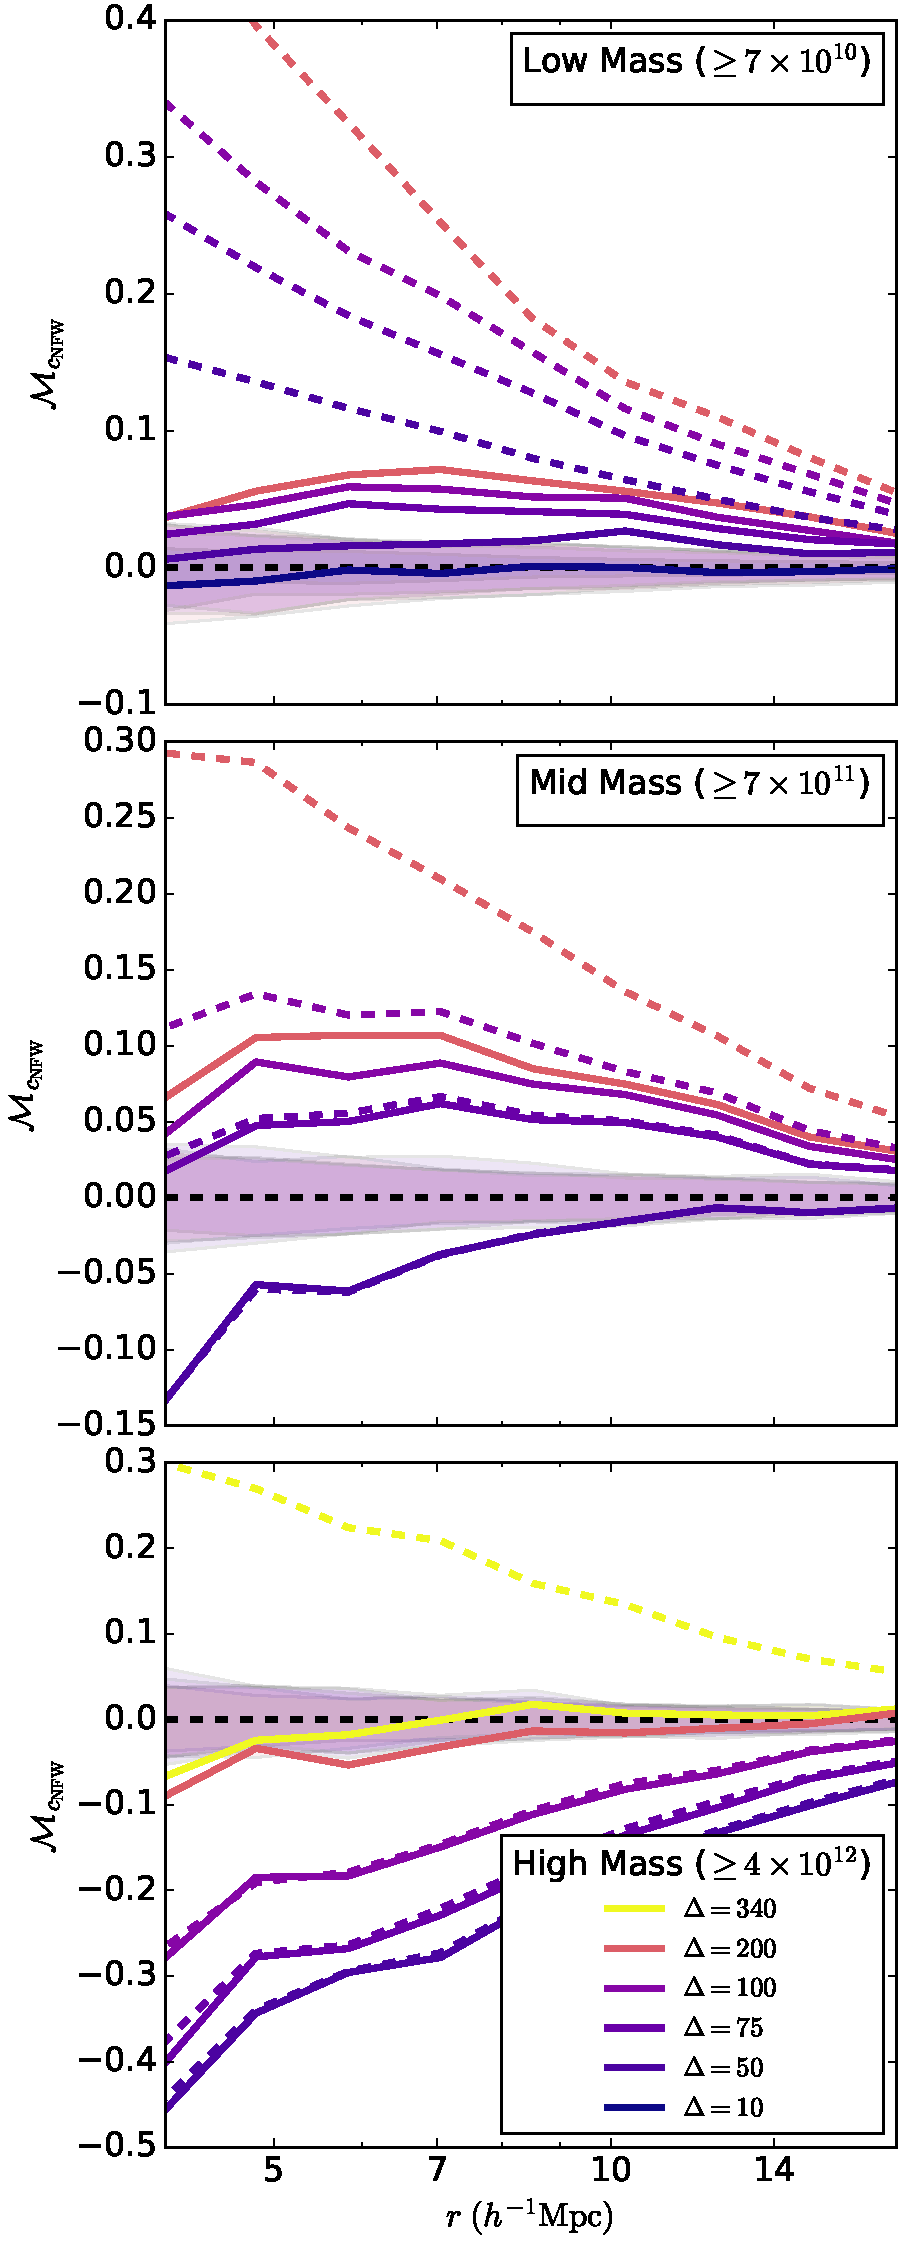
\includegraphics[width=.4\textwidth]{match_mcf_cNFW.pdf}
	\caption{The marked correlation function for the concentration defined according to the NFW profile. From top to bottom we show the `low mass', `mid mass', and `high mass' cutoffs. Only host halos consistent with the best-fit catalog from above are included in the analysis.}
	\label{fig:hvm_mcf_cnfw}
\end{figure}

\arz{Please check to ensure that I know what you mean by your matched samples. Your language was not 
specific enough for me to be 100\% sure. Modify as necessary.}
Figure~\ref{fig:hvm_mcf_cnfw} shows the same statistic as Figure~\ref{fig:cc_mcf_cnfw}, except for matched
subsamples. The matched subsamples are matched to a catalog generated for the value of $\Delta$ most likely to
remove assembly bias at large scales for the concentration marks; $\Delta=10$ for the `low mass' cut, $\Delta=70$
for the `mid mass' cut, and $\Delta=200$ for the `high mass' cut. These matched halo catalogs only differ from
the standard halo samples in that they contain only those host halos common 
to both the catalog in question and the best fit $\Delta$ catalog. The most interesting matched sample to 
examine in this case is the $\Delta=200$ sample. In this sample, all halos are defined as they would be 
defined in the $\Delta=200$ catalog, including all inferred halo properties; however, the matched catalog 
contains only those host halos that also appear in the $\Delta=70$ halo catalog. Therefore, many host 
halos have been removed from the sample because they have become subhalos in the $\Delta=70$ 
catalogs. 

From Fig.~\ref{fig:hvm_mcf_cnfw}, it is apparent that some degree of assembly bias persists in the matched 
samples. Yet, what is interesting is that a very significant fraction of the assembly bias effect has been 
removed compared to the standard $\Delta=200$ result. The halos in the matched catalogs have the 
same properties (including $c_{\mathrm{NFW}}$) as those in the standard catalogs, so that removal 
of assembly bias is {\em not} due to introducing noise or other systematics into the measurement of 
concentration. That mitigation of assembly bias is due to the halo redefinition and, in particular, 
subsuming those halos most subject to assembly bias effects as subhalos of the $\Delta=70$ 
halos. This is an interesting result suggesting that seeking optimal halo definitions may be 
one avenue to more completely separating the strongly nonlinear evolution occurring within 
halos from large-scale evolution and mitigating assembly bias. 


\begin{figure}
	\centering
	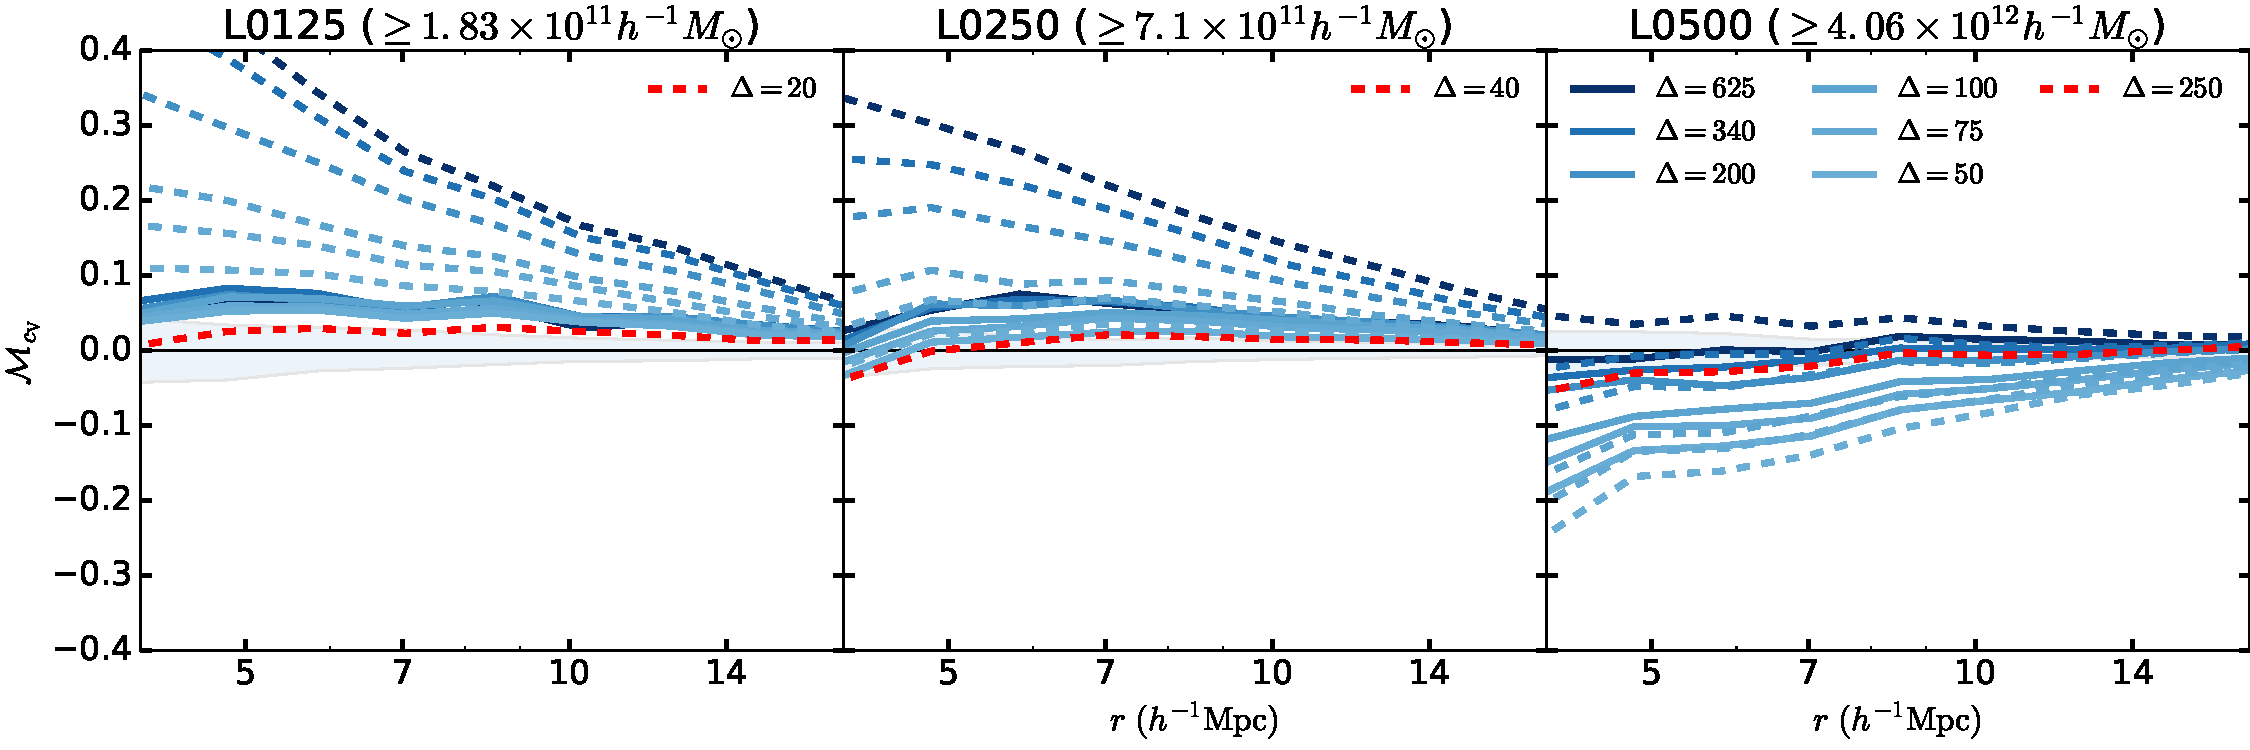
\includegraphics[width=.4\textwidth]{match_mcf_cV.pdf}
	\caption{
	\arz{All the same comments as for the $c_{\mathrm{NFW}}$ figure.}
	The marked correlation function for the concentration defined according to the velocity ratio. From top to bottom we show the `low mass', `mid mass', and `high mass' cutoffs. Only host halos consistent with the best-fit catalog from above are included in the analysis.}
	\label{fig:hvm_mcf_cV}
\end{figure}

\arz{Put a discussion of Fig.~\ref{fig:hvm_mcf_cV} here. It does not need to reiterate the discussion of 
Fig.~\ref{fig:hvm_mcf_cnfw}. However, it should state that we reach the same broad conclusion and that 
this is good in part because $c_{\mathrm{V}}$ is a nonparametric measure of halo concentration.}
Figure~\ref{fig:hvm_mcf_cV} follows the same exercise as above, with a comparison drawn to the Fig.~\ref{fig:cc_mcf_cV}. Notice that the same trends as Fig.~\ref{fig:hvm_mcf_cnfw} can be seen: a significant fraction of assembly bias is removed as compared to the unmatched catalog, though statistically significant assembly bias remains. Only in combination with halo redefinition do we remove assembly more completely on large scales.


\arz{Would it be easy for you to plot the concentration-mass relation for only those host halos 
in the ``matched" $\Delta=200$ sample? If so, that would be potentially interesting for our 
interpretation.}\asv{In progress for above.}

\arz{This paragraph is good, but needs to be written a bit more professionally. Start with a sentence like, 
``It is interesting to explore the reasons that halo shape, spin, and satellite number are not amenable 
to having their assembly bias mitigated through simple halo redefinitions." Then move on to some specifics.}
\asv{attempted to rewrite more professionally!}

While halo shape, spin, and satellite number are not amenable to having their assembly bias mitigated through the
simple halo redefinition technique we have suggested, the underlying reasons for this behavior remains of
interest for exploration. In the case of halo shape, we suggest that the assembly bias may be driven through
interactions with large scale structure. Studies have shown a statistically significant alignment between
filaments and satellite galaxy position \citep{tempel15, velliscig15}\asv{need to grab paper from arxiv
2016.05.09 for this}. Figure~\ref{fig:plotcircles} demonstrates the distribution of halos for the $\Delta=200$
and $\Delta=10$ catalogs of \simB. \asv{should probably remake this with halotools results just to be robust}
Notice the preferential distribution of satellites being subsumed into host halos.  Notice the preferential
direction in which host halos are subsumed in the latter definition. This material is likely to have significant
impact on the measurement of halo shape, potentially driving our results. This would also impact the satellite
number count, as the most clustered regions will see the largest increase as a result of this halo radius change.

\begin{figure*}
	\centering
	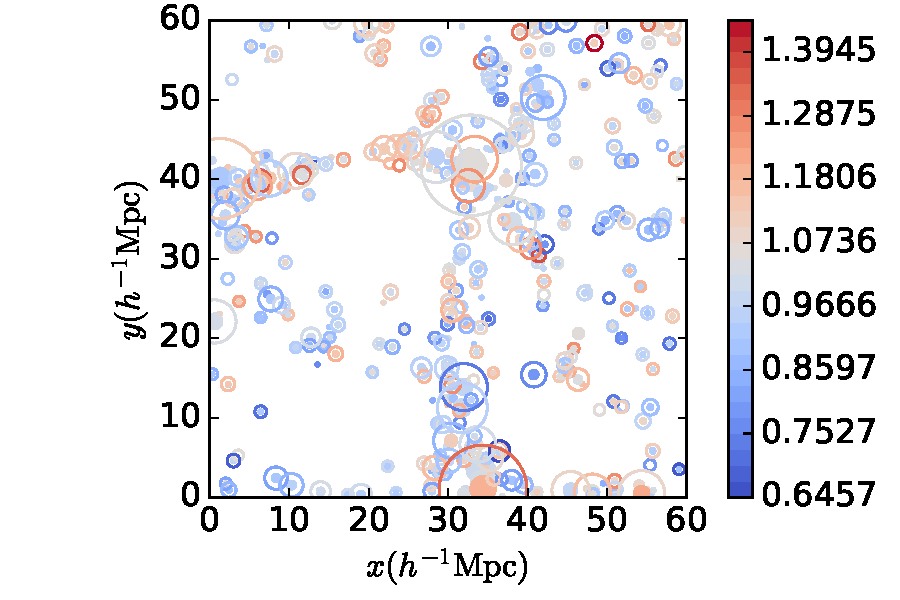
\includegraphics[width=.9\textwidth]{plotcircles.pdf}
	\caption{A $20 \hMpc$ deep cut of \simB \ along the z-axis. This zoom-in demonstrates the process that decreases the shape parameter as a function of clustering. The size of each circle represents the projection of a spherical dark matter halo with a given halo radius onto the x-y plane. Filled circles use the $\Delta = 200$ catalog and unfilled circles use the $\Delta = 10$ catalog in order to make the effect more visible. Color scale refers to the shape mark, normalized by halos of the same mass.}
	\label{fig:plotcircles}
\end{figure*}

Note that the mass dependence of assembly bias is implicitly explored with our suite of simulations.
The nature of the MCFs emphasizes halos just above the threshold mass; e.g. \simA~ probes the smallest mass
halos, while \simB~ probes the largest mass halos. One single halo definition is insufficient to account for the
entirety of assembly bias across the entire mass range. However, it is clear that assembly bias can be a strong
function of halo definition at fixed halo mass. Meta-analysis of the literature remains difficult as a natural
consequence, as different choices in the process of defining a halo can lead to significantly different results.
\arz{Instead, add one summarizing paragraph here discussing the mass dependence of assembly bias. 
Emphasize that our findings suggest that the strength of assembly bias can be a strong function of halo 
definition and that this may already be making it difficult to compare the results of various different research 
groups using different halo definitions.}


%----------------------
\section[]{Conclusions}
\label{section:conclusions}
%----------------------

\arz{After dealing with the comments above, let's come back to rewriting the conclusions section.}
We have looked at how to use CFs and MCFs in order to analyze the environmental effects upon the properties of the halo. We have suggested a method of removing the mass dependence that is not subject to the small number statistics at large halo masses. Taking our various tests, we then apply a change to the threshold density $\Delta$ in an attempt to remove the effect that environment has upon these properties. We come to the following conclusions from our simulation data.

\begin{itemize}
	\item Our halo redefinition method does not cause any substantial breakdown in the ROCKSTAR halo finding
algorithm, though this may not be the case for every halo finding methodology. This is something that should be
considered prior to utilization of this method, unless working directly from particle data. As our initial halo
sizes and locations are determined through spherical overdensities, it cannot be assumed that starting from a FoF
grouping and then determining values through particle data directly will produce identical results. Similarly,
different cosmologies may remove environmental effects at different scales.

	\item When looking at the two-point correlation function, there appears to be a ``sweet spot'' that appears
to remove environmental effects the most efficiently. Going beyond that seems to reintroduce environmental
effects, possibly as an extreme side effect of halo exclusion.

	\item For our marked correlation functions we see that both proxies of concentration that we use as marks
show significant removal of environmental effects at large scales for similar values of the overdensity parameter
$\Delta$. In cases where one is only interested in the concentration of dark matter halos and large scales (or
correspondingly small values of k), this method will allow you to compensate for bias that environment could
introduce to calculations dependent upon the halo model. This may prove valuable for calculations such as that of
the shear power spectrum calculated through weak lensing.

	\item The environmental effects on the shape of the host halo and the satellite number of the host halo
cannot be removed regardless of the chosen redefinition of $\Delta$. We propose that this may be intrinsically
tied to the nature of the filaments, whose effects cannot be removed by a simple redefinition of the halo radius.

	\item This method is definitively related to the mass of the halos that are being observed. Furthermore, it
appears that the majority of the reduction in assembly bias is tied to the exclusion of halos from the catalog as
a result of being subsumed into larger halos. This information does not seem to be contradictory; it can be
intuitively understood that the region about the most massive halos will be different than the region around the
least massive halos, leading to a different frequency at which halos are being excluded. It does however warrant
that careful consideration be given to the sample of halos that are of interest.

	\item The selection of halo size is intrinsically related to the assembly bias and varies across scales. This
might help to resolve contradictory results in the search for halo assembly bias in the literature.
\end{itemize}

This methodology, while certainly not perfect in accounting for assembly bias, may be of significance when
applied to galaxy formation models and give insight into seemingly conflicting results. Provided that the
properties of interest in a given model behave well under our redefinition, it will allow us to create better
mock galaxy catalogs without resorting to more complicated models requiring halo formation histories - giving us
another powerful tool to test observation against.

There remain possible uncertainties to study in the future. One possible area of follow-up is the matter of
simulation cosmology, which is not explored in this text. It is possible that the choice of cosmology may change
observed assembly bias as a function of the halo masses, something that our methodology should be capable of
observing. Furthermore, we can determine if the choice of halo size that best reduces assembly bias is a function
of the chosen cosmology. This may be of interest in attempting to determine signatures of assembly bias in
observational samples in the future.

\section*{Acknowledgments}

We are grateful to many people.

%%\bibliographystyle{plainnat}
\bibliography{master}

\section*{Appendix}
\label{section:appendix_massres}

One natural question that might arise in the analysis of this work is the nature of the resulting assembly bias
trends. Our focus in the main sections of this paper is on the nature of the assembly bias changing as a function
of the mass cut chosen. Our conclusions include the fact that there is a strong mass dependence on halo assembly
bias that must be accounted for seperately depending on the halos of interest in a study. However, while the
existence of this trend is clear within our analysis, the determination that this is solely due to the masses of
the halos included in our calculation is less clear upon closer inspection. One possibility that might be
particularly concerning is the potential that the different simulations have created halos that have
fundamentally different clustering and this is leading to the result that we are interpreting as a mass
dependence on assembly bias. Thankfully, though our statistics become less meaningful to carry out this
calculation, we can carry out a comparison using the same mass cut across two of our simulations, knowing that
these will only contain well resolved halos.

While not addressed directly, Figure~\ref{fig:hvl_cfcompare} through Figure~\ref{fig:hvl_mcf_nsat} contain a
demonstration of the result that we are seeking in the left column of panels. The lower left panels show various
marks of interest for \simB \ using the ``mid mass'' cut on the data set. In comparison, the upper left panel
contains the same marks of interest for the \simA \ using the same mass cut. In the latter, there are fewer halos
in this mass cut range, as a result of the smaller simulation box size. However, we note that despite the
additional noise in the data set, the behavior of the assembly bias measurement is nearly identical within
tolerances accounting for differences between simulations and noise. This motivates our conclusion that the
driver behind the behavior is the mass cut of the data sets rather than the resolution of the simulation.

\label{lastpage}

\end{document}
